%File: formatting-instructions-latex-2026.tex
%release 2026.0
\documentclass[letterpaper]{article} % DO NOT CHANGE THIS
\usepackage{aaai2026}  % DO NOT CHANGE THIS
\usepackage{times}  % DO NOT CHANGE THIS
\usepackage{helvet}  % DO NOT CHANGE THIS
\usepackage{courier}  % DO NOT CHANGE THIS
\usepackage[hyphens]{url}  % DO NOT CHANGE THIS
\usepackage{graphicx} % DO NOT CHANGE THIS
\urlstyle{rm} % DO NOT CHANGE THIS
\def\UrlFont{\rm}  % DO NOT CHANGE THIS
\usepackage{natbib}  % DO NOT CHANGE THIS AND DO NOT ADD ANY OPTIONS TO IT
\usepackage{caption} % DO NOT CHANGE THIS AND DO NOT ADD ANY OPTIONS TO IT
\usepackage{booktabs}
% \usepackage{xcolor}
\usepackage{multirow}
\usepackage{amssymb}
\usepackage{pifont}
\usepackage{enumitem}
\usepackage{tabularx}

\frenchspacing  % DO NOT CHANGE THIS
\setlength{\pdfpagewidth}{8.5in}  % DO NOT CHANGE THIS
\setlength{\pdfpageheight}{11in}  % DO NOT CHANGE THIS
%
% These are recommended to typeset algorithms but not required. See the subsubsection on algorithms. Remove them if you don't have algorithms in your paper.
\usepackage{algorithm}
\usepackage{algorithmic}
\usepackage[table,xcdraw]{xcolor}

%
% These are are recommended to typeset listings but not required. See the subsubsection on listing. Remove this block if you don't have listings in your paper.
\usepackage{newfloat}
\usepackage{listings}
\DeclareCaptionStyle{ruled}{labelfont=normalfont,labelsep=colon,strut=off} % DO NOT CHANGE THIS
\lstset{%
	basicstyle={\footnotesize\ttfamily},% footnotesize acceptable for monospace
	numbers=left,numberstyle=\footnotesize,xleftmargin=2em,% show line numbers, remove this entire line if you don't want the numbers.
	aboveskip=0pt,belowskip=0pt,%
	showstringspaces=false,tabsize=2,breaklines=true}
\floatstyle{ruled}
\newfloat{listing}{tb}{lst}{}
\floatname{listing}{Listing}
%
% Keep the \pdfinfo as shown here. There's no need
% for you to add the /Title and /Author tags.
\pdfinfo{
/TemplateVersion (2026.1)
}

% DISALLOWED PACKAGES
% \usepackage{authblk} -- This package is specifically forbidden
% \usepackage{balance} -- This package is specifically forbidden
% \usepackage{color (if used in text)
% \usepackage{CJK} -- This package is specifically forbidden
% \usepackage{float} -- This package is specifically forbidden
% \usepackage{flushend} -- This package is specifically forbidden
% \usepackage{fontenc} -- This package is specifically forbidden
% \usepackage{fullpage} -- This package is specifically forbidden
% \usepackage{geometry} -- This package is specifically forbidden
% \usepackage{grffile} -- This package is specifically forbidden
% \usepackage{hyperref} -- This package is specifically forbidden
% \usepackage{navigator} -- This package is specifically forbidden
% (or any other package that embeds links such as navigator or hyperref)
% \indentfirst} -- This package is specifically forbidden
% \layout} -- This package is specifically forbidden
% \multicol} -- This package is specifically forbidden
% \nameref} -- This package is specifically forbidden
% \usepackage{savetrees} -- This package is specifically forbidden
% \usepackage{setspace} -- This package is specifically forbidden
% \usepackage{stfloats} -- This package is specifically forbidden
% \usepackage{tabu} -- This package is specifically forbidden
% \usepackage{titlesec} -- This package is specifically forbidden
% \usepackage{tocbibind} -- This package is specifically forbidden
% \usepackage{ulem} -- This package is specifically forbidden
% \usepackage{wrapfig} -- This package is specifically forbidden
% DISALLOWED COMMANDS
% \nocopyright -- Your paper will not be published if you use this command
% \addtolength -- This command may not be used
% \balance -- This command may not be used
% \baselinestretch -- Your paper will not be published if you use this command
% \clearpage -- No page breaks of any kind may be used for the final version of your paper
% \columnsep -- This command may not be used
% \newpage -- No page breaks of any kind may be used for the final version of your paper
% \pagebreak -- No page breaks of any kind may be used for the final version of your paperr
% \pagestyle -- This command may not be used
% \tiny -- This is not an acceptable font size.
% \vspace{- -- No negative value may be used in proximity of a caption, figure, table, section, subsection, subsubsection, or reference
% \vskip{- -- No negative value may be used to alter spacing above or below a caption, figure, table, section, subsection, subsubsection, or reference

\setcounter{secnumdepth}{2} %May be changed to 1 or 2 if section numbers are desired.

% The file aaai2026.sty is the style file for AAAI Press
% proceedings, working notes, and technical reports.
%

% Title
% \newcommand{\equalcontrib}{\textsuperscript{*}Equal contribution}

% Your title must be in mixed case, not sentence case.
% That means all verbs (including short verbs like be, is, using,and go),
% nouns, adverbs, adjectives should be capitalized, including both words in hyphenated terms, while
% articles, conjunctions, and prepositions are lower case unless they
% directly follow a colon or long dash
\title{AirCopBench: A Benchmark for Multi-drone Collaborative \\
Embodied Perception and Reasoning}
\author{
    %Authors
    % All authors must be in the same font size and format.
    Jirong Zha \textsuperscript{\rm 1}\textsuperscript{*$\blacklozenge$}, Yuxuan Fan\textsuperscript{\rm 2}\textsuperscript{*},
    Tianyu Zhang\textsuperscript{\rm 3}, Geng Chen\textsuperscript{\rm 4}, 
    \\
    Yingfeng Chen\textsuperscript{\rm 5}, Chen Gao\textsuperscript{\rm 6 \dag}, Xinlei Chen\textsuperscript{\rm 1 \dag}
    % Marc Pujol-Gonzalez\equalcontrib
}
\affiliations{
    %Afiliations
    \textsuperscript{\rm 1}Shenzhen International Graduate School, Tsinghua University \\
    \textsuperscript{\rm 2}The Hong Kong University of Science and Technology (Guang Zhou) \\
    \textsuperscript{\rm 3}School of Electrical and Electronic Engineering, Nanyang Technological University \\
    \textsuperscript{\rm 4}College of Software, Jilin University \\
    \textsuperscript{\rm 5}Weiyang College, Tsinghua University \\
    \textsuperscript{\rm 6}BNRist, Tsinghua University \\
    zhajirong23@mails.tsinghua.edu.cn, yfan546@connect.hkust-gz.edu.cn,
    tianyu016@e.ntu.edu.sg,
    chengeng0201@gmail.com,
    chenying24@mails.tsinghua.edu.cn,
    chgao96@gmail.com,
    chen.xinlei@sz.tsinghua.edu.cn \\
    \textsuperscript{*} Equal Contribution.
    \textsuperscript{$\blacklozenge$} Project Leader.
    \textsuperscript{\dag} Corresponding Authors.
}

% \footnotetext[1]{Corresponding author}

%Example, Single Author, ->> remove \iffalse,\fi and place them surrounding AAAI title to use it
\iffalse
\title{My Publication Title --- Single Author}
\author {
    Author Name
}
\affiliations{
    Affiliation\\
    Affiliation Line 2\\
    name@example.com
}
\fi

\iffalse
%Example, Multiple Authors, ->> remove \iffalse,\fi and place them surrounding AAAI title to use it
\title{My Publication Title --- Multiple Authors}
\author {
    % Authors
    First Author Name\textsuperscript{\rm 1,\rm 2},
    Second Author Name\textsuperscript{\rm 2},
    Third Author Name\textsuperscript{\rm 1}
}
\affiliations {
    % Affiliations
    \textsuperscript{\rm 1}Affiliation 1\\
    \textsuperscript{\rm 2}Affiliation 2\\
    firstAuthor@affiliation1.com, secondAuthor@affilation2.com, thirdAuthor@affiliation1.com
}
\fi


% REMOVE THIS: bibentry
% This is only needed to show inline citations in the guidelines document. You should not need it and can safely delete it.
% \usepackage{bibentry}
% END REMOVE bibentry

\begin{document}

\makeatletter % Allows us to use commands with "@" in their name

\twocolumn[{%
\begin{center}
    % These \vskip commands are copied from the aaai2026.sty file to match the official title spacing.
    \vskip 0.625in minus 0.125in

    % Manually typesetting the title
    {\LARGE\bf \@title \par}%

    \vskip 0.1in plus 0.5fil minus 0.05in

    % --- FIX ---
    % We must manually define \theauthors here because we are not calling \maketitle.
    % This definition is copied directly from aaai2026.sty to ensure it correctly
    % handles the [submission] option.
    \def\theauthors{\if T\showauthors@on\@author\else Anonymous submission\fi}

    % Now, we typeset the authors using our local definition of \theauthors.
    {\Large{\textbf{\theauthors}}\par}%

    \vskip .2em plus 0.25fil

    % Manually typesetting the affiliations
    {\normalsize \affiliations_\par}%

    \vskip 1em plus 2fil

    % --- Your Figure Goes Here ---
    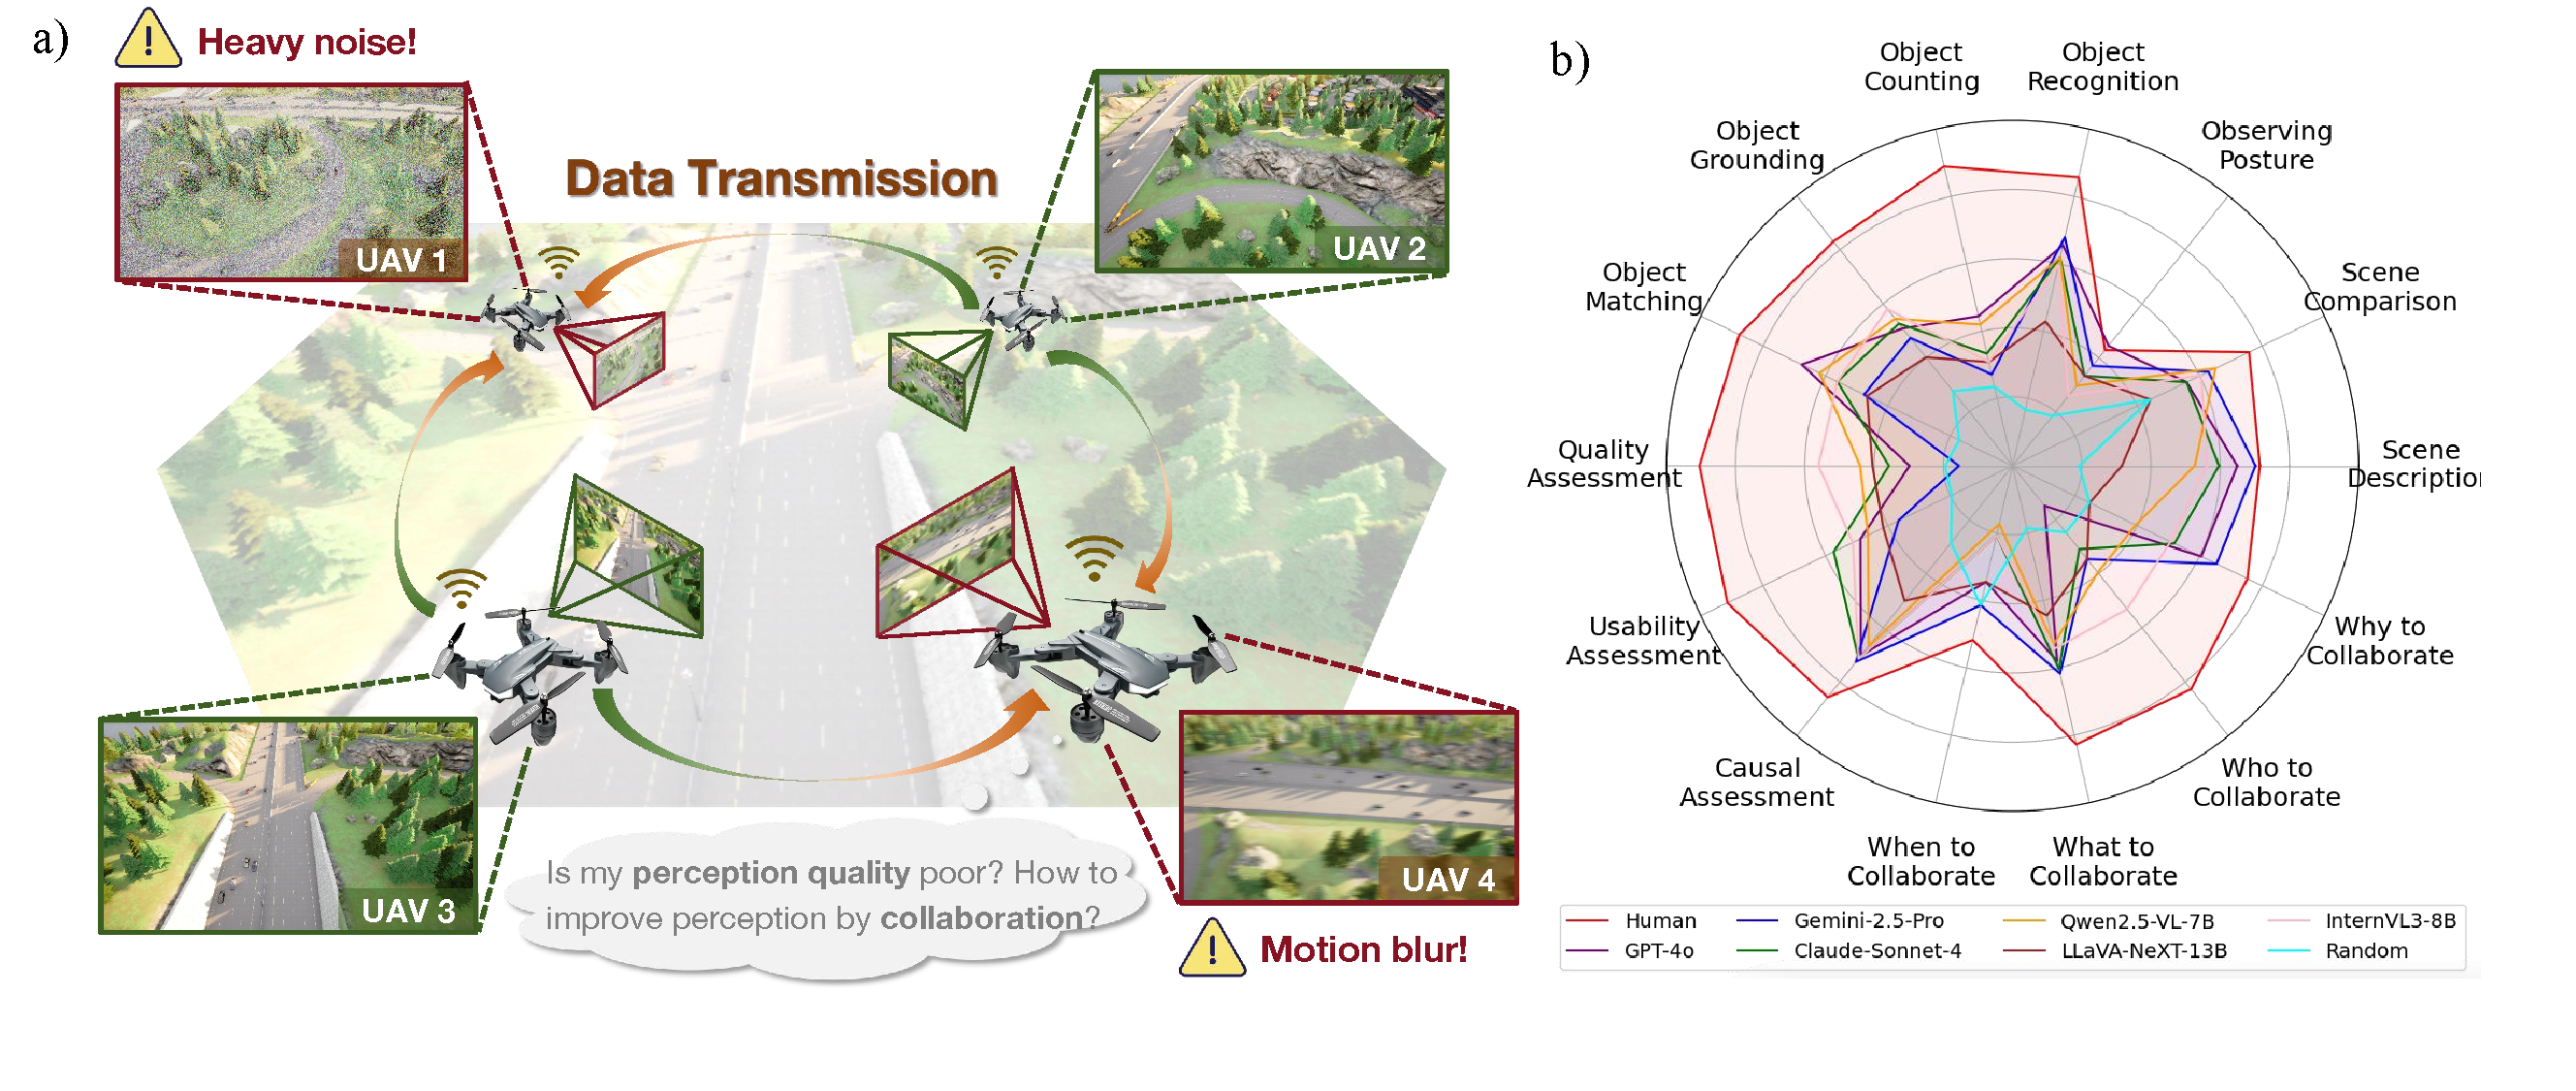
\includegraphics[width=1\linewidth]{figures/overview.pdf}
    % Use \captionof from the 'caption' package for non-floating figures
    \captionof{figure}{a) Illustration of multi-drone collaborative perception with various perception degradation. b) The performance of 6 popular MLLMs, along with human and random guess baselines, on AirCopBench.}
    \label{intro}
\end{center}
}]

\makeatother


% \maketitle

\begin{abstract}
Multimodal Large Language Models (MLLMs) have shown promise in single-agent vision tasks, yet benchmarks for evaluating multi-agent collaborative perception remain scarce. This gap is critical, as multi-drone systems provide enhanced coverage, robustness, and collaboration compared to single-sensor setups. Existing multi-image benchmarks mainly target basic perception tasks using high-quality single-agent images, thus failing to evaluate MLLMs in more complex, egocentric collaborative scenarios, especially under real-world degraded perception conditions.To address these challenges, we introduce AirCopBench, the first comprehensive benchmark designed to evaluate MLLMs in embodied aerial collaborative perception under challenging perceptual conditions. AirCopBench includes 14.6k+ questions derived from both simulator and real-world data, spanning four key task dimensions: Scene Understanding, Object Understanding, Perception Assessment, and Collaborative Decision, across 14 task types. 
We construct the benchmark using data from challenging degraded-perception scenarios with annotated collaborative events, generating large-scale questions through model-, rule-, and human-based methods under rigorous quality control. Evaluations on 40 MLLMs show significant performance gaps in collaborative perception tasks, with the best model trailing humans by 24.38\% on average and exhibiting inconsistent results across tasks. Fine-tuning experiments further confirm the feasibility of sim-to-real transfer in aerial collaborative perception and reasoning.
\end{abstract}

% Uncomment the following to link to your code, datasets, an extended version or similar.
% You must keep this block between (not within) the abstract and the main body of the paper.
\begin{links}
\vspace{-0.3cm}
    % \link{Code}{https://github.com/zhajirong/AirCopBench}
    % \link{Dataset}{https://aaai.org/example/datasets}
    \link{Project}{https://embodiedcity.github.io/AirCopBench/}
    % \link{Appendix}{https://aaai.org/example/extended-version}
    \vspace{-0.3cm}
\end{links}

\begin{table*}[t]
\centering
\caption{Comparison of the proposed and popular benchmarks for collaborative perception.}
\resizebox{\textwidth}{!}
{
\begin{tabular}{lcccccccc}
\toprule
\textbf{Benchmark} & \textbf{Modality} & \textbf{Object Category} & \textbf{Perception Degradation} & \textbf{VQA} & \textbf{VQA Num.} & \textbf{Embodied} \\ 
\midrule
Coperception-UAV \cite{hu2022where2comm} & RGB & Vehicles & / & \ding{55} & / & \ding{51} \\
MDMT \cite{liu2023robust} & RGB & Vehicles, bicycles, pedestrians & Occlusion, lighting, blur & \ding{55} & / & \ding{51} \\
UAV3D \cite{sunderraman2024uav3d} & RGB & Vehicles & / & \ding{55} & / & \ding{51} \\
AeroCollab3D \cite{tian2024ucdnet} & RGB & Vehicles, pedestrians & / & \ding{55} & / & \ding{51} \\
Air-Co-Pred \cite{wang2024drones} & RGB & Vehicles, bicycles, pedestrians & Occlusion, long distance & \ding{55} & / & \ding{51} \\
MUIRBENCH \cite{wang2024muirbench} & RGB, text & Vehicles, buildings & Occlusion & \ding{51} & 2.6k & \ding{55}\\
All-Angles Bench \cite{yeh2025seeing} & RGB, text & Pedestrians & Occlusion & \ding{51} & 2.1k & \ding{55} \\
UrBench \cite{zhou2025urbench} & RGB, text & Vehicles, buildings & / & \ding{51} & 11.6k & \ding{55} \\
% \rowcolor{gray!20}
\midrule
\multirow{2}{*}{Our AirCopBench} & RGB, text, & Drones, vehicles, bicycles, & Occlusion, shadow, noise, lighting, out of FoV,  & \multirow{2}{*}{\ding{51}} & \multirow{2}{*}{14.6k} & \multirow{2}{*}{\ding{51}} \\
 & point cloud & pedestrians & data loss, long distance/small target, blur &  & \\
\bottomrule
\end{tabular}
}
\label{comparison}
\end{table*}

\section{Introduction}

Multimodal Large Language Models (MLLMs) have transformed artificial intelligence (AI) by enabling powerful processing of diverse inputs, such as text and images \cite{caffagni2024revolution, zhang2024mm, fu2024blink}. While MLLMs have excelled in single-agent vision tasks like object detection and semantic segmentation \cite{saini2025advancing, zang2025contextual, huang2025mllm}, as well as general multi-image understanding tasks \cite{cheng2025evaluating, bai2025hallucination}, their performance in collaborative perception with multiple unmanned aerial vehicles (UAVs) remains underexplored. In multi-UAV systems, drones work together to tackle complex, dynamic visual tasks through information exchange, offering enhanced coverage, robustness, and flexibility compared to single-agent configurations \cite{liu2020when2com, zha2024diffusion, lin2025mcop}.

Despite the potential of multi-UAV systems, benchmarks evaluating MLLMs in collaborative perception are scarce. Current evaluations focus primarily on single-agent vision tasks, failing to address the unique challenges of multi-UAV collaborative perception, such as obstacle occlusion \cite{kil2024mllm, xiao2025uav, guo2025bedi, chen2025large}.
% This gap limits our understanding of how MLLMs perform when multiple UAVs collaborate to share and synthesize information in real-world settings. 
Furthermore, existing benchmarks on collaborative perception \cite{wang2024drones, tian2024ucdnet, liu2020when2com} in Tab.~\ref{comparison} face two major limitations that hinder their applicability in adaptive real-world scenarios:
% Moreover, current aerial collaborative perception benchmarks also lack challenging perception degradation types and fail to account for embodied reasoning for context-aware perception and decision-making, making them less applicable to adaptive real-world applications.
%
% Current evaluation benchmarks for multimodal systems have predominantly focused on single-agent perception tasks, typically involving high-quality, static images. While these benchmarks have been essential for advancing the state of the art in AI, they do not capture the complexities and challenges of real-world scenarios, particularly in multi-agent collaboration. One key limitation of these existing benchmarks is their failure to simulate the conditions that multi-agent systems encounter in practical applications. For instance, the degradation of perception quality due to environmental factors—such as low-light conditions, obstructions, or sensor malfunctions—is rarely considered. Furthermore, these benchmarks typically overlook the need for collaborative strategies where multiple agents must not only perceive their individual surroundings but also share and synthesize information to achieve collective goals.
%
%
% Multi-agent collaborative perception has gained significant attention in areas such as autonomous driving \cite{han2023collaborative} and urban surveillance \cite{naik2024bucktales}, owing to its superior coverage and robustness compared to single-agent observation systems \cite{liu2020when2com}. Recent advancements in Unmanned Aerial Vehicle (UAV) technologies have further highlighted the relevance of multi-UAV systems for collaborative perception tasks including object detection, environment mapping, and situational awareness \cite{sunderraman2024uav3d}. Multi-UAV collaborative perception enables the coordination of multiple UAVs that exchange diverse perspectives and data. This collaboration enhances the multi-UAV system's overall accuracy and reliability, particularly in handling object occlusion scenarios \cite{wang2024drones}. 
% By leveraging the diverse perspectives and data from multiple UAVs, this strategy helps overcome the limitations faced by individual UAVs, providing a more robust solution, particularly in complex and dynamic environments.
%

%
% Existing research on multi-UAV collaborative perception 
% %, such as When2com, Where2comm, and How2comm, 
% primarily focuses on balancing the tradeoff between transmission bandwidth and perception performance \cite{yu2025which2comm, hu2024communication, where2comm, liu2020when2com}. 
% % with limited perception degradation scenarios and .
% However, two key challenges still exist, limiting the full collaboration potential of multi-UAV perception and restricting their effectiveness in real-world applications.
%
% Moreover, existing research on multi-UAV collaborative perception \cite{yu2025which2comm, hu2024communication, where2comm, liu2020when2com} often oversimplifies perception scenarios and multi-UAV collaboration strategies, leading to two key limitations towards challenging real-world collaborative perception tasks:

% However, existing research on multi-UAV collaborative perception \cite{yu2025which2comm, hu2024communication, where2comm, liu2020when2com} often oversimplifies perception scenarios and multi-UAV collaboration strategies, leading to two key issues that limit the method's applicability to challenging real-world collaborative perception tasks:
% and a lack of relevant datasets and evaluation metrics for challenging collaborative perception applications.

% However, two key challenges remain, limiting the full collaboration potential of multi-UAV perception and hindering their effectiveness in real-world applications. Existing approaches \cite{yu2025which2comm, hu2024communication, where2comm, liu2020when2com} oversimplify perception scenarios and multi-agent collaboration, resulting in a lack of relevant datasets and evaluation metrics for challenging real-world applications.

\begin{itemize}[left=0pt]
    % \item Various Perception Degradation in Real-world Scenarios: 
    \item \textit{Oversimplified Perception Setups}:
    Despite occlusion, numerous factors such as sensor noise, poor visibility, data loss, and environmental interference can degrade the quality of UAVs' observation data, thus reducing overall perception accuracy. Current benchmarks consider only a limited set of degradation types, restricting their adaptability to real-world conditions.

    % Factors such as sensor noise, poor visibility, and environmental interference can degrade the data quality captured by UAVs, which compromise the accuracy of individual UAVs’ perception and consequently influence the performance of the entire observation system. Current methods only consider limited perception degradation types with a lot of focus on occlusion and often fail to adapt to these real-world scenarios, limiting the application adaptability of methods.
    % The challenge lies in how to efficiently and effectively mitigate these issues by fully leveraging the collaborative advantages of the UAVs to overcome perception degradation. Current methods often fail to adapt to these real-world imperfections in a way that optimizes collaboration and improves overall performance.
    
    % \item  Lack of Egocentric Reasoning and Adaptive Decision-making: 
    \item  \textit{Lack of Embodied Reasoning}: 
    Aerial collaborative perception demands rich semantic information processing and highly adaptive cooperation in complex environments. Traditional non-egocentric, programmatic decision-making schemes, based on global data fusion, hinder UAVs from making context-aware, human-like, first-view decisions, limiting their ability to understand their state, adapt to changes, and collaborate efficiently.
    % Without egocentric reasoning, UAVs cannot assess their own state or context, limiting adaptive behavior. Combined with rigid decision-making, this leads to inflexible strategies that fail in dynamic environments. UAVs struggle to interpret and respond to shared data, hindering effective collaboration. The lack of both egocentric reasoning and decision-making flexibility prevents context-aware, intelligent choices, particularly in complex or ambiguous situations.

    % Without egocentric reasoning, UAVs are unable to assess their own state or context, hindering their ability to adapt their behavior effectively. This, combined with rigid, programmatic decision-making, results in inflexible strategies that are not suitable for dynamic environments. UAVs struggle to interpret and respond to the meaning of shared data in real-time, leading to suboptimal collaboration. The absence of both egocentric reasoning and flexibility in decision-making prevents UAVs from making intelligent, context-aware choices, especially in complex or ambiguous scenarios.
\end{itemize}
%
Therefore, it is essential to assess MLLMs' cognitive abilities in embodied perception and collaborative decision-making under challenging perceptual conditions, as illustrated in Fig.~\ref{intro}. More related work can be found in \textit{Appendix}.
% In this context, each UAV first evaluates its own image quality, identifies degradation causes, and determines optimal collaboration strategies with other UAVs, as illustrated in Fig.~\ref{intro}.
% Therefore, there is an urgent need to explore embodied aerial collaborative perception under challenging perceptual conditions, where each UAV first assesses its own image quality, identifies the causes of perception degradation, and then determines optimal collaboration strategies with other UAVs, as depicted in Fig.~\ref{intro}. 

% Recent advancements in Multimodl Large Language Models (MLLMs) \cite{zhang2024mm} offer potential solutions for embodied perception and adaptive collaboration. Models like GPT-4o \cite{hurst2024gpt} and Gemini \cite{comanici2025gemini} excel in visual reasoning and semantic interaction, making them ideal for complex environment analysis. However, benchmarks for MLLMs in aerial collaborative perception remain scarce. 
%
% Integrating MLLMs into multi-UAV systems improves context-aware understanding and the efficiency of collaborative perception in real-world scenarios. 
% Thus, evaluating MLLMs' cognitive capabilities in embodied perception and decision-making is crucial for advancing multi-UAV perception.

% Recent advancements in Multimodal Large Language Models (MLLMs) \cite{zhang2024mm} offer promising solutions for embodied perception assessment and adaptive collaboration decision-making in various perception degradation scenarios. Models like GPT-4o \cite{hurst2024gpt}, Gemini \cite{comanici2025gemini}, and LLaVA \cite{liu2024llava} excel in vision-based tasks, autonomous reasoning, and semantic interaction, making them effective for analyzing and reasoning in complex environments. However, benchmarks for MLLMs in aerial collaborative perception are scarce, particularly those addressing diverse constrained perceptual conditions.
% Integrating MLLMs into multi-UAV systems enhances context-aware understanding and analysis, improving the accuracy and efficiency of collaborative perception, especially in real-world scenarios with perception degradation. 
% Thus, evaluating MLLMs' embodied cognitive capabilities in perception assessment and collaborative decision-making can provide valuable insights for future multi-UAV perception.

% Therefore, there is a urgent need for research on embodied aerial collaborative perception with various challenging perception degradation. 
% Recent advancements in Multi-Modal Large Models (MLLMs) offer promising solutions for intelligent embodied collaborative perception in perception-degraded scenarios. MLLMs have demonstrated impressive performance in vision-based tasks and are capable of autonomous reasoning and semantic interaction, especially effective for analysis and reasoning in complex scenarios with perception degradation, which are crucial for overcoming the limitations outlined above. 
% Integrating MLLMs into multi-UAV systems enables improved decision-making, adaptive collaboration, and meaningful semantic interactions. 
% By integrating MLLMs into multi-UAV collaborative systems, UAVs can better reason through complex scenarios, engage in meaningful semantic interactions, and make adaptive, intelligent decisions based on context. From this, we infer that assessing MLLMs' embodied cognitive abilities offers insights for future collaborative perception applications. 

% To address these challenges, recent advancements in Multi-Modal Large Models (MLLMs) offer promising solutions. MLLMs have demonstrated impressive performance in vision-based tasks and are capable of autonomous reasoning and semantic interaction.
% , which are crucial for overcoming the limitations outlined above. 

Accordingly, we propose \textbf{AirCopBench}, a novel benchmark designed to evaluate MLLMs in multi-UAV collaborative perception under various challenging perception conditions. Specifically, we introduce an innovative task set comprising 14 tasks across 4 dimensions from simultaneous multi-view images. Our dataset includes challenging data from both simulators \cite{gao2024embodiedcity, hu2022where2comm, tian2024ucdnet} and real world \cite{liu2023robust}, collected from diverse UAV groups in representative degraded scenarios.
% and capturing observations of different targets
% in representative degraded scenarios. 
% To simulate additional degradation factors such as sensor failures and data loss, we apply image post-processing techniques like noise injection and partial masking. 
Besides traditional object-level labeling for perception tasks, we incorporate event-level labeling by human annotators for specific cooperation events. Then, we develop a general pipeline to generate high-quality visual question answering (VQA) pairs using model-based, rule-based, and human-based approaches, followed by stringent quality control measures, including standard review, blind filtering, and human refinement.
%
Finally, we evaluate our dataset on popular MLLMs in zero-shot settings, including both proprietary and open-source models, and conduct supervised fine-tuning (SFT) on Qwen2.5-series \cite{bai2025qwen2} and LLaVA-NeXT series \cite{liu2024llavanext} to validate the dataset's effectiveness. The results show that current MLLMs struggle with multi-view collaborative perception, exhibiting inconsistent performance across different task types.
% In our framework, each UAV first assesses its own image quality, identifies the causes of perception degradation, and then determines optimal collaboration strategies with other UAVs. 
%
\begin{figure*}[t]
    \centering
    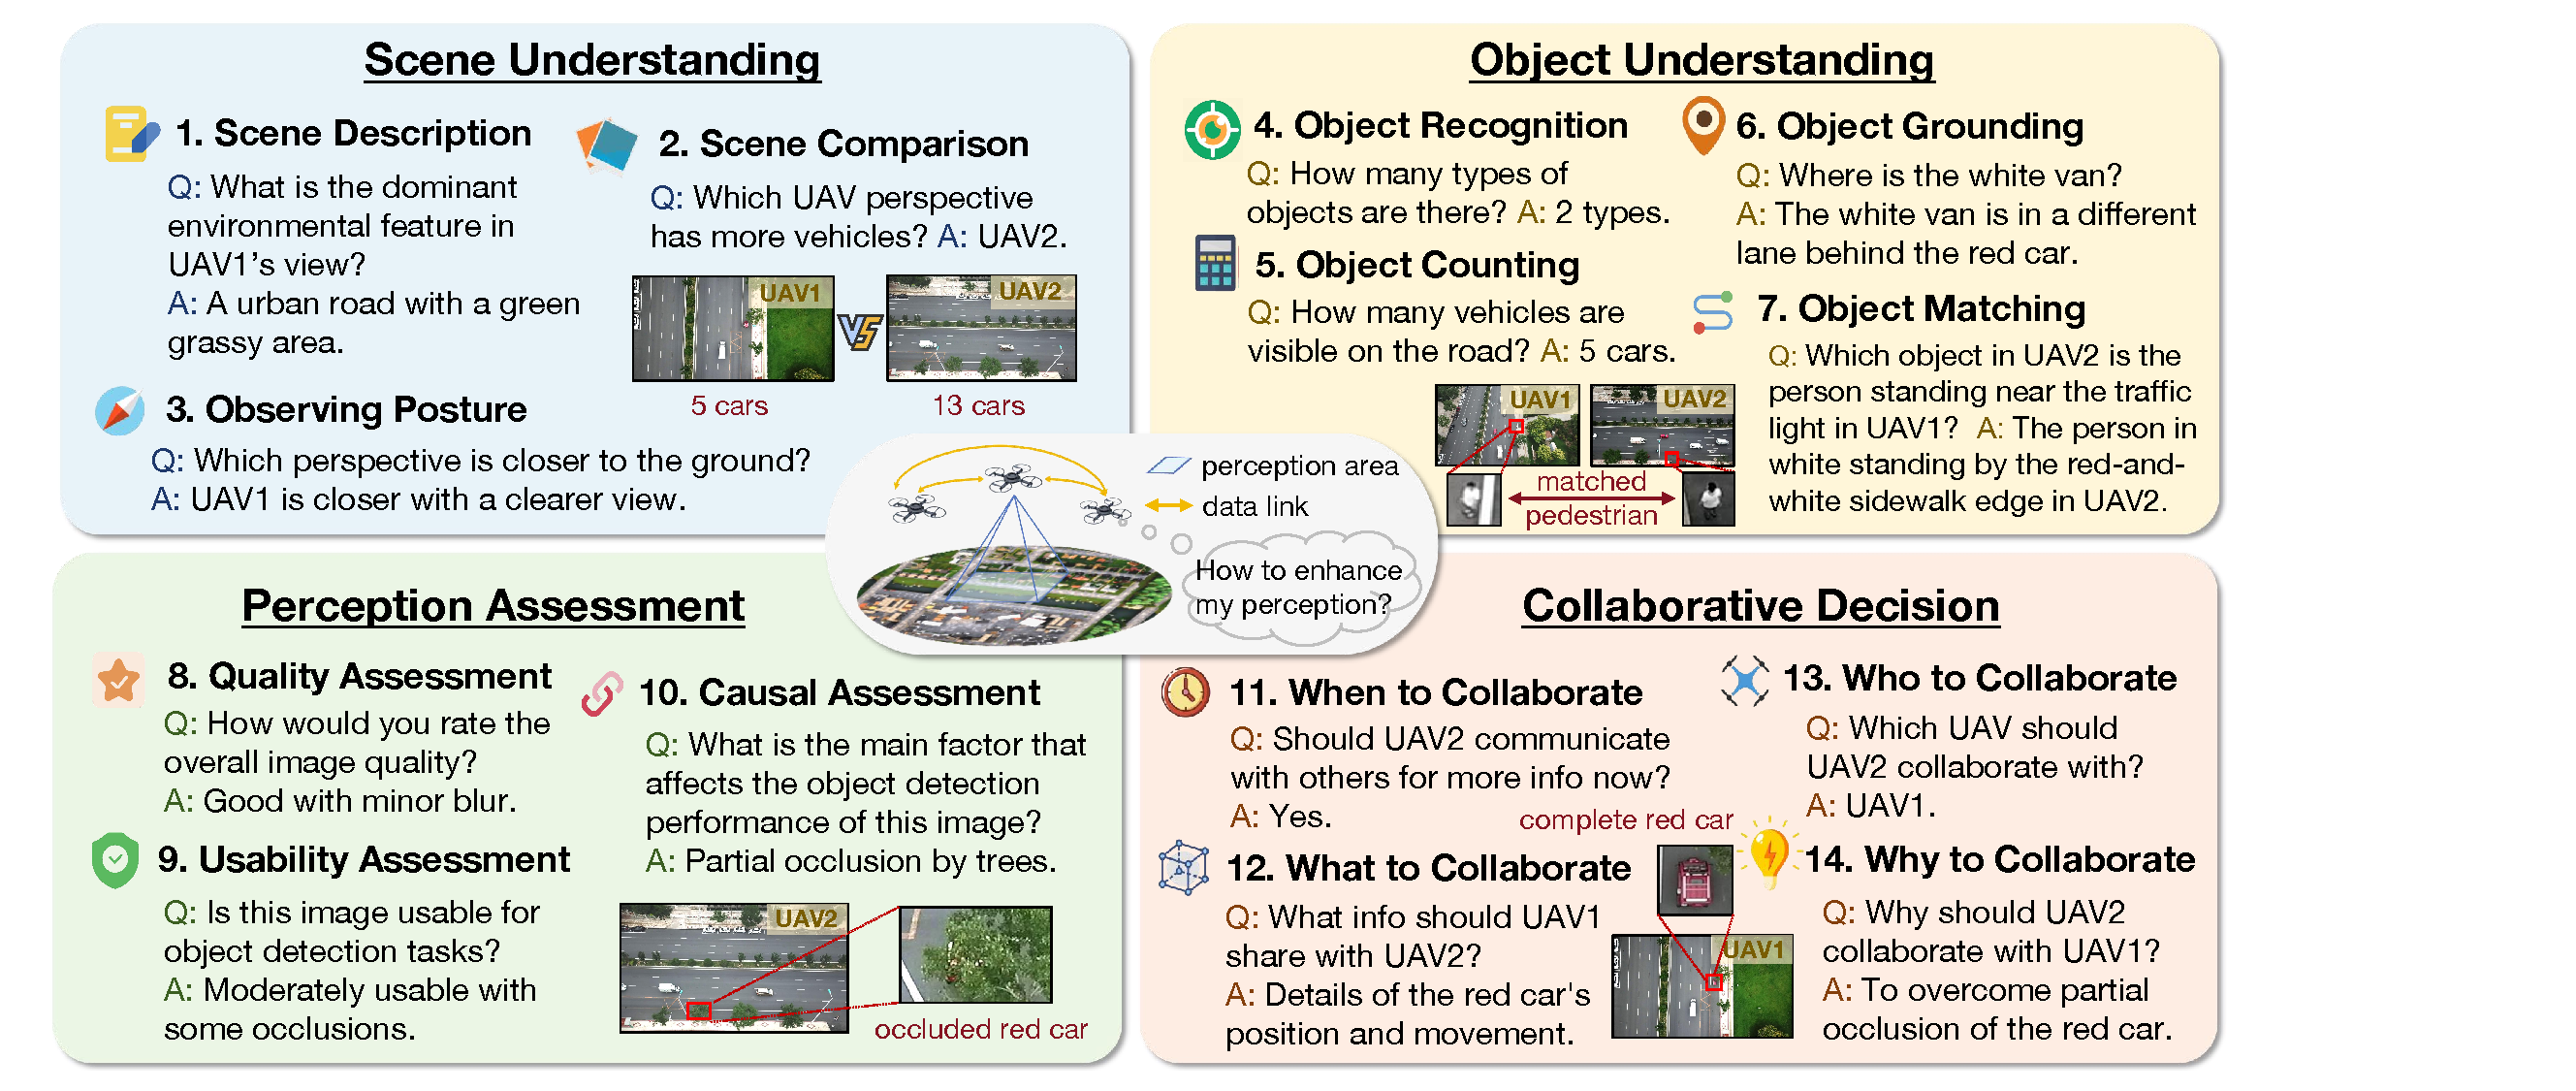
\includegraphics[width=0.92\linewidth]{figures/task.pdf}
    \caption{AirCopBench includes 14 task types across 4 evaluation dimensions: Scene Understanding, Object Understanding, Perception Assessment, and Collaborative Decision. This categorization facilitates a systematic evaluation of MLLMs, from image understanding and quality analysis to multi-UAV information exchange for improved collaborative embodied perception.}
    \label{task}
    \vspace{-0.3cm}
\end{figure*}

Compared to existing aerial collaborative perception benchmarks, key features of AirCopBench include: 
1) Semantic VQA pairs to evaluate MLLMs’ ability in perception assessment and collaborative reasoning;
2) Various challenging perception degradation in real-world scenarios, such as occlusion, shadows, motion blur, noise, data loss, long-range detection, complex background, etc;
3) Multiple modalities, including RGB images, text, and point clouds, to support perception across diverse data types;
4) Diverse target categories, covering drones, pedestrians, vehicles, and bicycles;
5) Embodied multi-UAV collaboration from first-view, role-based reasoning for human-like decision-making. 

% 1) Semantic VQA for collaborative Reasoning: AirCopBench uses interactive, semantic Visual Question Answering (VQA) pairs to assess MLLMs’ ability to collaboratively reason and solve complex multi-UAV perception tasks;
% b) Challenging Perception Conditions: 
% AirCopBench considers various real-world perception challenges, such as occlusion, shadows, noise, data loss, long-range detection, time variations, weather changes, etc;
% c) Multiple Modalities: 
% AirCopBench includes RGB images, text, and point clouds to test the model's ability to process and reason across diverse data types;
% d) Diverse Target Categories: AirCopBench evaluates perception for a wide range of targets, including aerial objects, pedestrians, vehicles, and bicycles;
% e) Embodied Multi-UAV Collaboration: 
% AirCopBench emphasizes role-based reasoning in multi-UAV tasks, testing models on their ability to collaborate and make decisions in dynamic environments.

Overall, the novelty of this research lies in creating \textbf{the first benchmark for semantic embodied aerial collaborative perception considering various challenging perception degradation}. Our contributions are fourfold:
\begin{itemize}[left=0pt]
    \item We introduce a novel task set with 4 categories and 14 tasks to evaluate MLLMs' abilities in scene and object understanding, perception assessment, and collaborative decision-making using multi-view images.
    \item We create an aerial collaborative perception dataset with over 2.9k+ multi-view images from UAV groups of varying sizes, annotated for collaborative events, and focused on diverse perception degradations.
    \item We construct 14.6k+ VQA pairs from collaborative UAV observations using both real and simulated data, and design an extensible benchmark pipeline applicable to other multi-view embodied settings.
    \item We evaluate 40 MLLMs and investigate the relationship between embodied collaborative perception tasks and Sim-to-Real potential. We also fine-tune 4 models to demonstrate the effectiveness of our dataset.
\end{itemize}


\section{AirCopBench}

AirCopBench is a high-quality aerial perception benchmark with 14 tasks across 4 dimensions, including challenging perception degradation scenarios. Based on quantitative multi-view images from various drone groups, it evaluates MLLMs' embodied collaborative perception capabilities. This section outlines the task definitions, generation pipeline, and statistical properties of the benchmark.

% AirCopBench is a high-quality aerial perception benchmark featuring 14 tasks across 4 dimensions, incorporating challenging perception degradation scenarios. Built from quantitative multi-view images captured by various drone groups, 
% % both in simulators and the real world, 
% AirCopBench is designed to assess the embodied collaborative perception capabilities of MLLMs. This section provides an overview of the task definitions, generation pipeline, and statistical properties of the benchmark.

% \subsection{Benchmark Overview}
% \subsubsection{Dataset Statistics.} 
% As detailed in Fig.3, UrBench comprises 2K+ images, 11.6K questions, which are divided into a validation set for hyperparameter selection and a test set for evaluation. The validation set and the test set contain approximately 1.1K and 10.5K questions, respectively. Please refer to the Appendix for further statistical details.



\subsection{Benchmark Tasks}

AirCopBench includes four key task dimensions: Scene Understanding, Object Understanding, Perception Assessment, and Collaborative Decision. Each category is further divided into sub-tasks to enable a more detailed evaluation of MLLMs' capabilities, as shown in Fig.~\ref{task}.

% To comprehensively assess MLLMs' collaborative perception capabilities under challenging sensory conditions, we design 4 key task categories: Scene Understanding, Object Understanding, Perception Assessment, and Collaborative Decision. Each key task is further divided into several sub-tasks to enrich the dataset and provide a clearer, finer-grained evaluation of MLLMs' capabilities in specialized areas, as shown in Fig.~\ref{task}. 

\subsubsection{Scene Understanding} refers to interpreting and understanding scenes from multi-view images (Task 1-3 in Fig.~\ref{task}). Specifically, Scene Description identifies objects, relationships, and context in one scene, while Scene Comparison reveals similarities and differences between images from different views \cite{zhou2025urbench}.
Observing Posture analyzes the relative distances and directions between observers and the scene, crucial for simulating human-like observations in embodied aerial perception tasks.

\subsubsection{Object Understanding} focuses on analyzing objects in terms of identity, quantity, and spatial relationships (Tasks 4-7 in Fig.~\ref{task}). Particularly, Object Recognition identifies object types, Object Counting determines object quantity for specific types, Object Grounding assesses the spatial positioning between objects, and Object Matching finds corresponding objects across different views \cite{zhou2025urbench}.

\subsubsection{Perception Assessment} evaluates image quality and usability for specific perception tasks (Task 8-10 in Fig.~\ref{task}). In detail, Quality Assessment rates image by objectively checking its clarity and resolution, while Usability Assessment subjectively determines its effectiveness for object detection. Causal Assessment traces the reasons for poor-quality or unsuitable images, analyzing whether degradation is due to sensor issues, moving targets, or environmental factors. This helps UAVs better understand their perception state and supports information exchange with other observing UAVs.

\begin{figure*}[t]
    \centering
    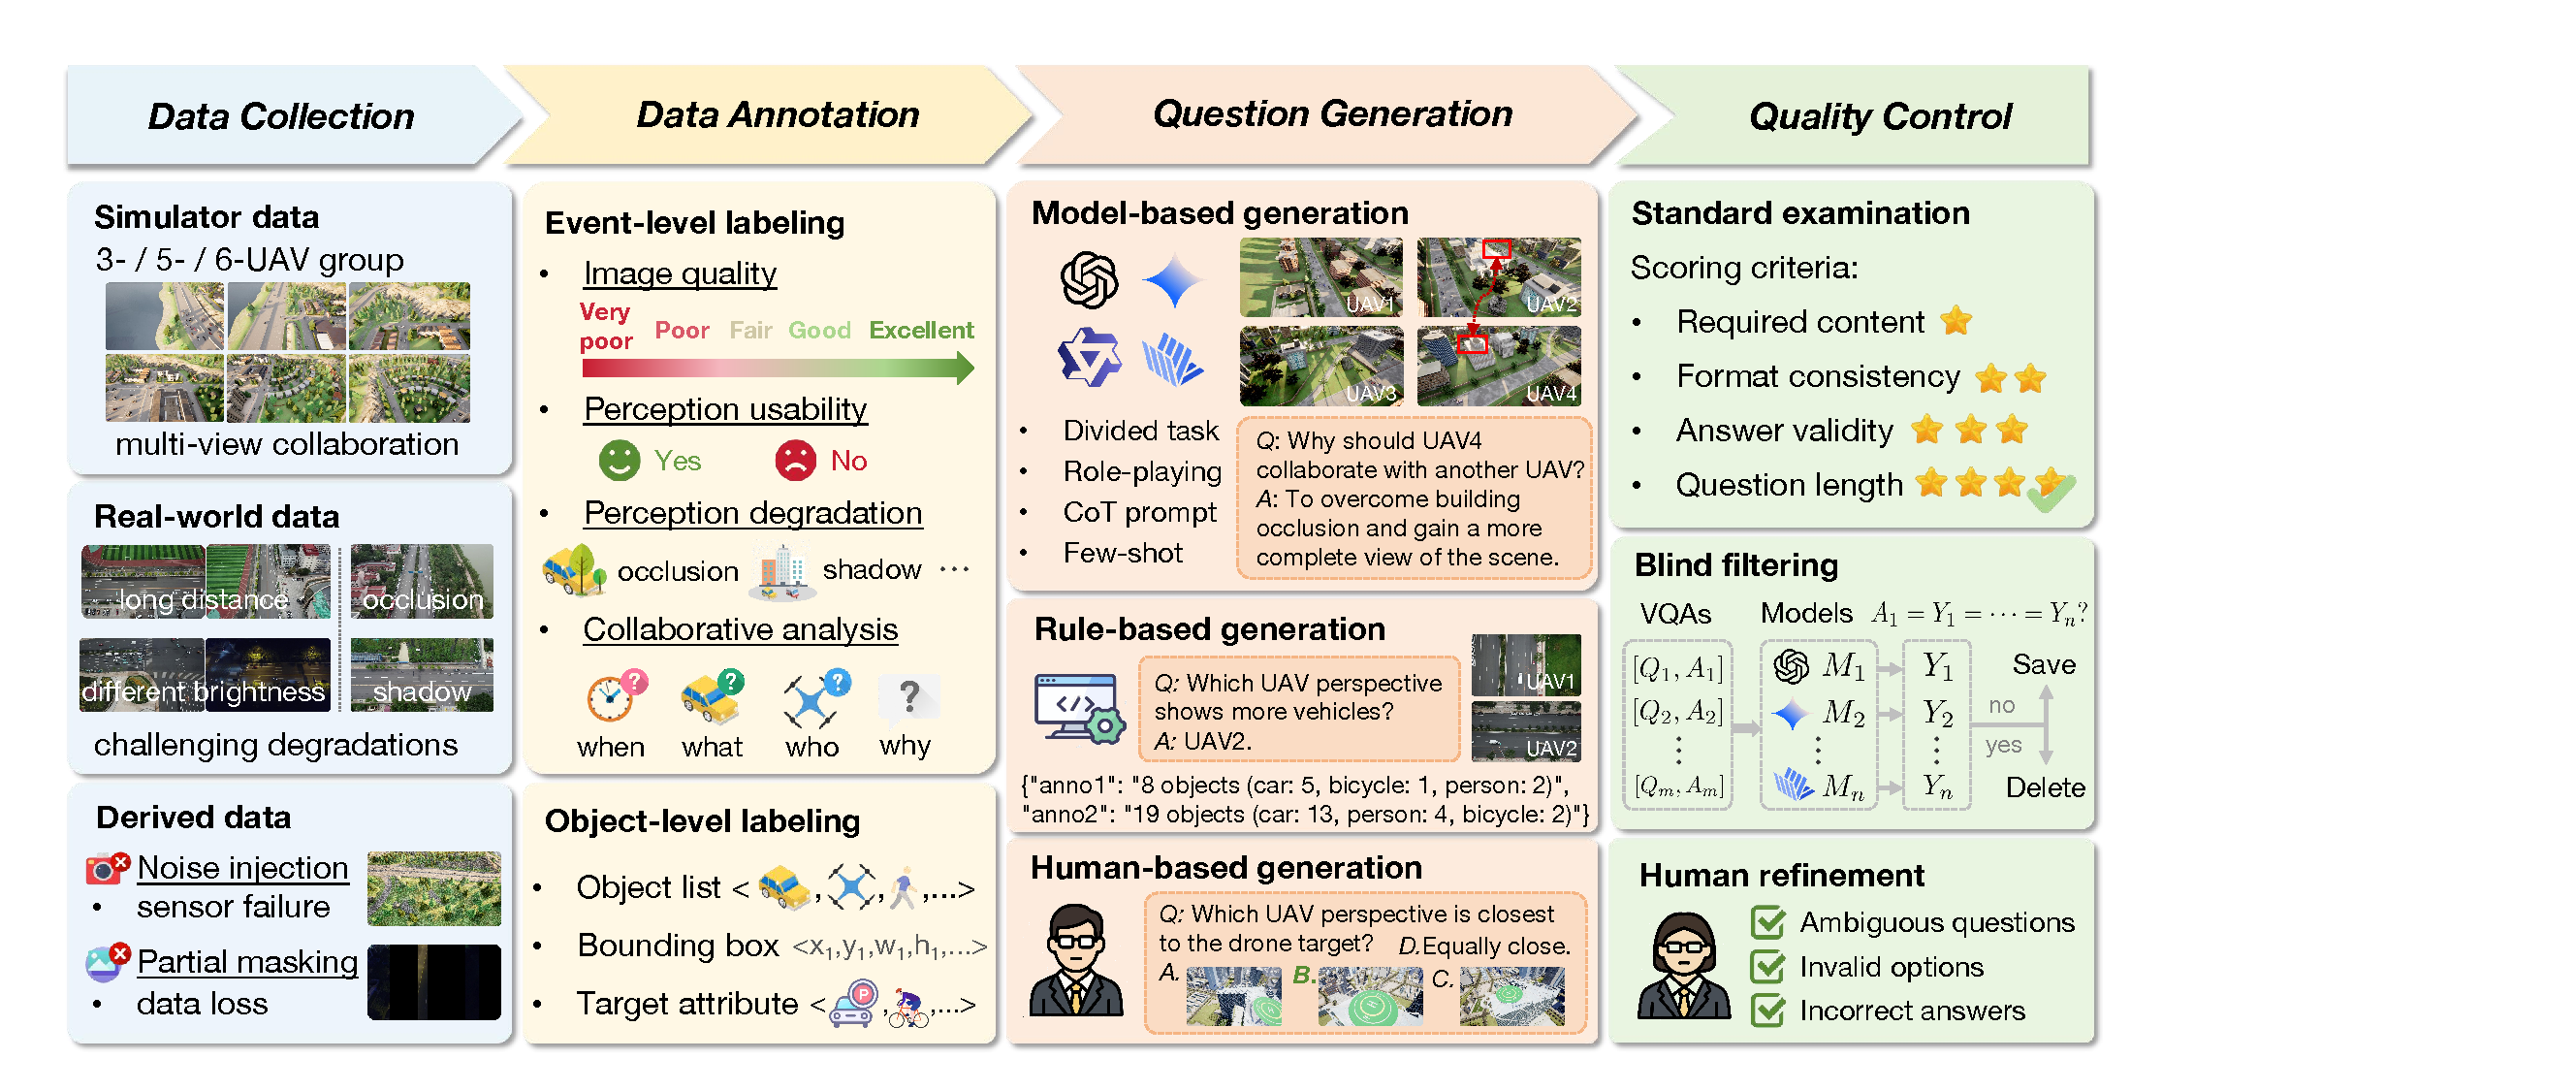
\includegraphics[width=0.95\linewidth]{figures/pipeline.pdf}
    \caption{AirCopBench generation pipeline includes 4 main steps: Data Collection, Data Annotation, Question Generation, and Quality Control. This systematic approach ensures the validity and high quality of the generated dataset.}
    \label{pipeline}
    \vspace{-0.3cm}
\end{figure*}

\subsubsection{Collaborative Decision} determines the need for information exchange among UAVs (Task 11-14 in Fig.~\ref{task}). 
% Tasks here examine when, what, who, and why collaboration with other UAVs is necessary (Task 11-14 in Fig.~\ref{task}). 
This task design aims to enhance collaboration efficiency between UAVs by reducing communication and computational costs of the multi-UAV system. 
Specifically, When to Collaborate identifies scenarios where collaboration is essential for current UAV, while What to Collaborate determines the information that should be shared between UAVs. Who to Collaborate assesses which UAVs are best suited for collaboration, and Why to Collaborate explores the motivations behind information exchange between UAVs. 


\subsection{Benchmark Generation}
The benchmark generation pipeline consists of four main steps: Data Collection, Data Annotation, Question Generation, and Quality Control, as illustrated in Fig.~\ref{pipeline}.

\subsubsection{Data Collection.}
To effectively evaluate MLLMs in challenging scenarios, high-quality data with realistic perception degradations, such as occlusion, shadow, noise, lighting imbalance, data loss, motion blur, long distance, and out-of-field of view (FoV), is essential.
% To effectively evaluate MLLMs in challenging scenarios, it is essential to collect high-quality data containing realistic perception degradation such as occlusion, shadow, noise, lighting imbalance, data loss, motion blur, long distance, diverse weather, and out of field of view (FoV), etc. 
% These challenges are key to testing MLLMs under degraded conditions. 
% As described in the Data Collection stage in Fig.~\ref{pipeline}, 
Our data consists of:
\\
\indent \textbf{Simulator Data.}
    Multimodal collaborative perception data, including RGB images and point clouds, is collected from co-simulated Carla \cite{dosovitskiy2017carla} and AirSim \cite{shah2017airsim}. This includes challenging ground vehicle target perception from 5-6 UAVs in existing datasets, Coperception-UAV \cite{hu2022where2comm} and AeroCollab3D \cite{tian2024ucdnet}, and drone target observation from 3 UAVs collected from EmbodiedCity \cite{gao2024embodiedcity}. The data spans 20 different map scenarios, focusing on those inducing key perceptual degradation issues, as detailed in \textit{Appendix}.
\\
\indent 
\textbf{Real-world Data.}
    To enhance data credibility, we select representative images from existing real-world dataset MDMT \cite{liu2023robust}, where 2 UAVs cooperatively perceive ground targets like vehicles, pedestrians, and bicycles. These scenarios include various perception challenges such as motion blur, varying lighting (day/night), distant small targets, and obstacle occlusions. 
    % Incorporating real-world data with perception degradation enhances the authenticity, diversity, and reliability of our dataset.
\\
\indent
\textbf{Derived Data.}
    To expand the dataset and introduce more perceptual degradation, we apply two image post-processing techniques:
    a) Noise Injection adds random noises (Gaussian, salt-and-pepper, impulse, Poisson) to simulate sensor failures;
    b) Partial Masking blocks part of the image to simulate visual information loss.
    These techniques simulate perception degradation scenarios, such as low signal-to-noise ratio (SNR) and data loss due to sensor damage or failures, that are hard to capture in simulators or real environments.
    % To expand the dataset and introduce additional perceptual degradation, we apply two image post-processing techniques: 
    % a) Noise Injection, which simulates sensor failures by adding random noises like Gaussian, salt-and-pepper, impulse, and Poisson noise; 
    % b) Partial Masking, which blocks part of the image to simulate visual information loss. 
    % These techniques help simulate more perceptual degradation scenarios, such as low signal-to-noise ratio (SNR) and data loss due to sensor damage or failure, that are difficult to capture in simulators or real-world environments.  

\subsubsection{Data Annotation.}
Rich, rational annotations tailored for aerial collaborative perception improve dataset accuracy and realism. In this work, we focus on both event-level labels, capturing inter-UAV collaboration, and object-level labels, ensuring precise identification in complex scenes.
\\ \indent
\textbf{Event-level Labeling.} To emphasize the role of collaboration in perception, we introduce novel ``event" annotations to assist in generating multi-UAV 
interaction strategies,  
% under degraded perception scenarios, 
such as when and why inter-UAV communication is needed, who is suitable for information retrieval, and what observation information should be shared. Despite labeling for collaborative decision analysis, the annotations in this part also include image quality scoring, perception usability assessment, and perception degradation reasoning for better event understanding. The whole manual annotation process costs over 200 hours. More details are in \textit{Appendix}.
\\ \indent
\textbf{Object-level Labeling.} Traditional annotations for object labeling involve the list of specified objects in the scene, the 2D/3D bounding box of each object, and the corresponding attributes of objects like motion state \cite{hu2022where2comm}. This enables accurate collaborative perception for targets, including target detection, classification, and tracking.


% \subsubsection{Data Annotation.}
% \begin{enumerate}[label=(\arabic*)]
%     \item Event Labelling: Image quality: excellent, good, fair, poor, very poor. Perception usability: yes or no. Perception degradation: occlusion, shadow, long distance, out of FoV, noise, loss, lighting. Collaborative analysis: when, what, who, why.

%     \item Traditional labelling: Object list. Bounding box. Target attribute.
 
% \end{enumerate}

\begin{figure*}[t]
    \centering
    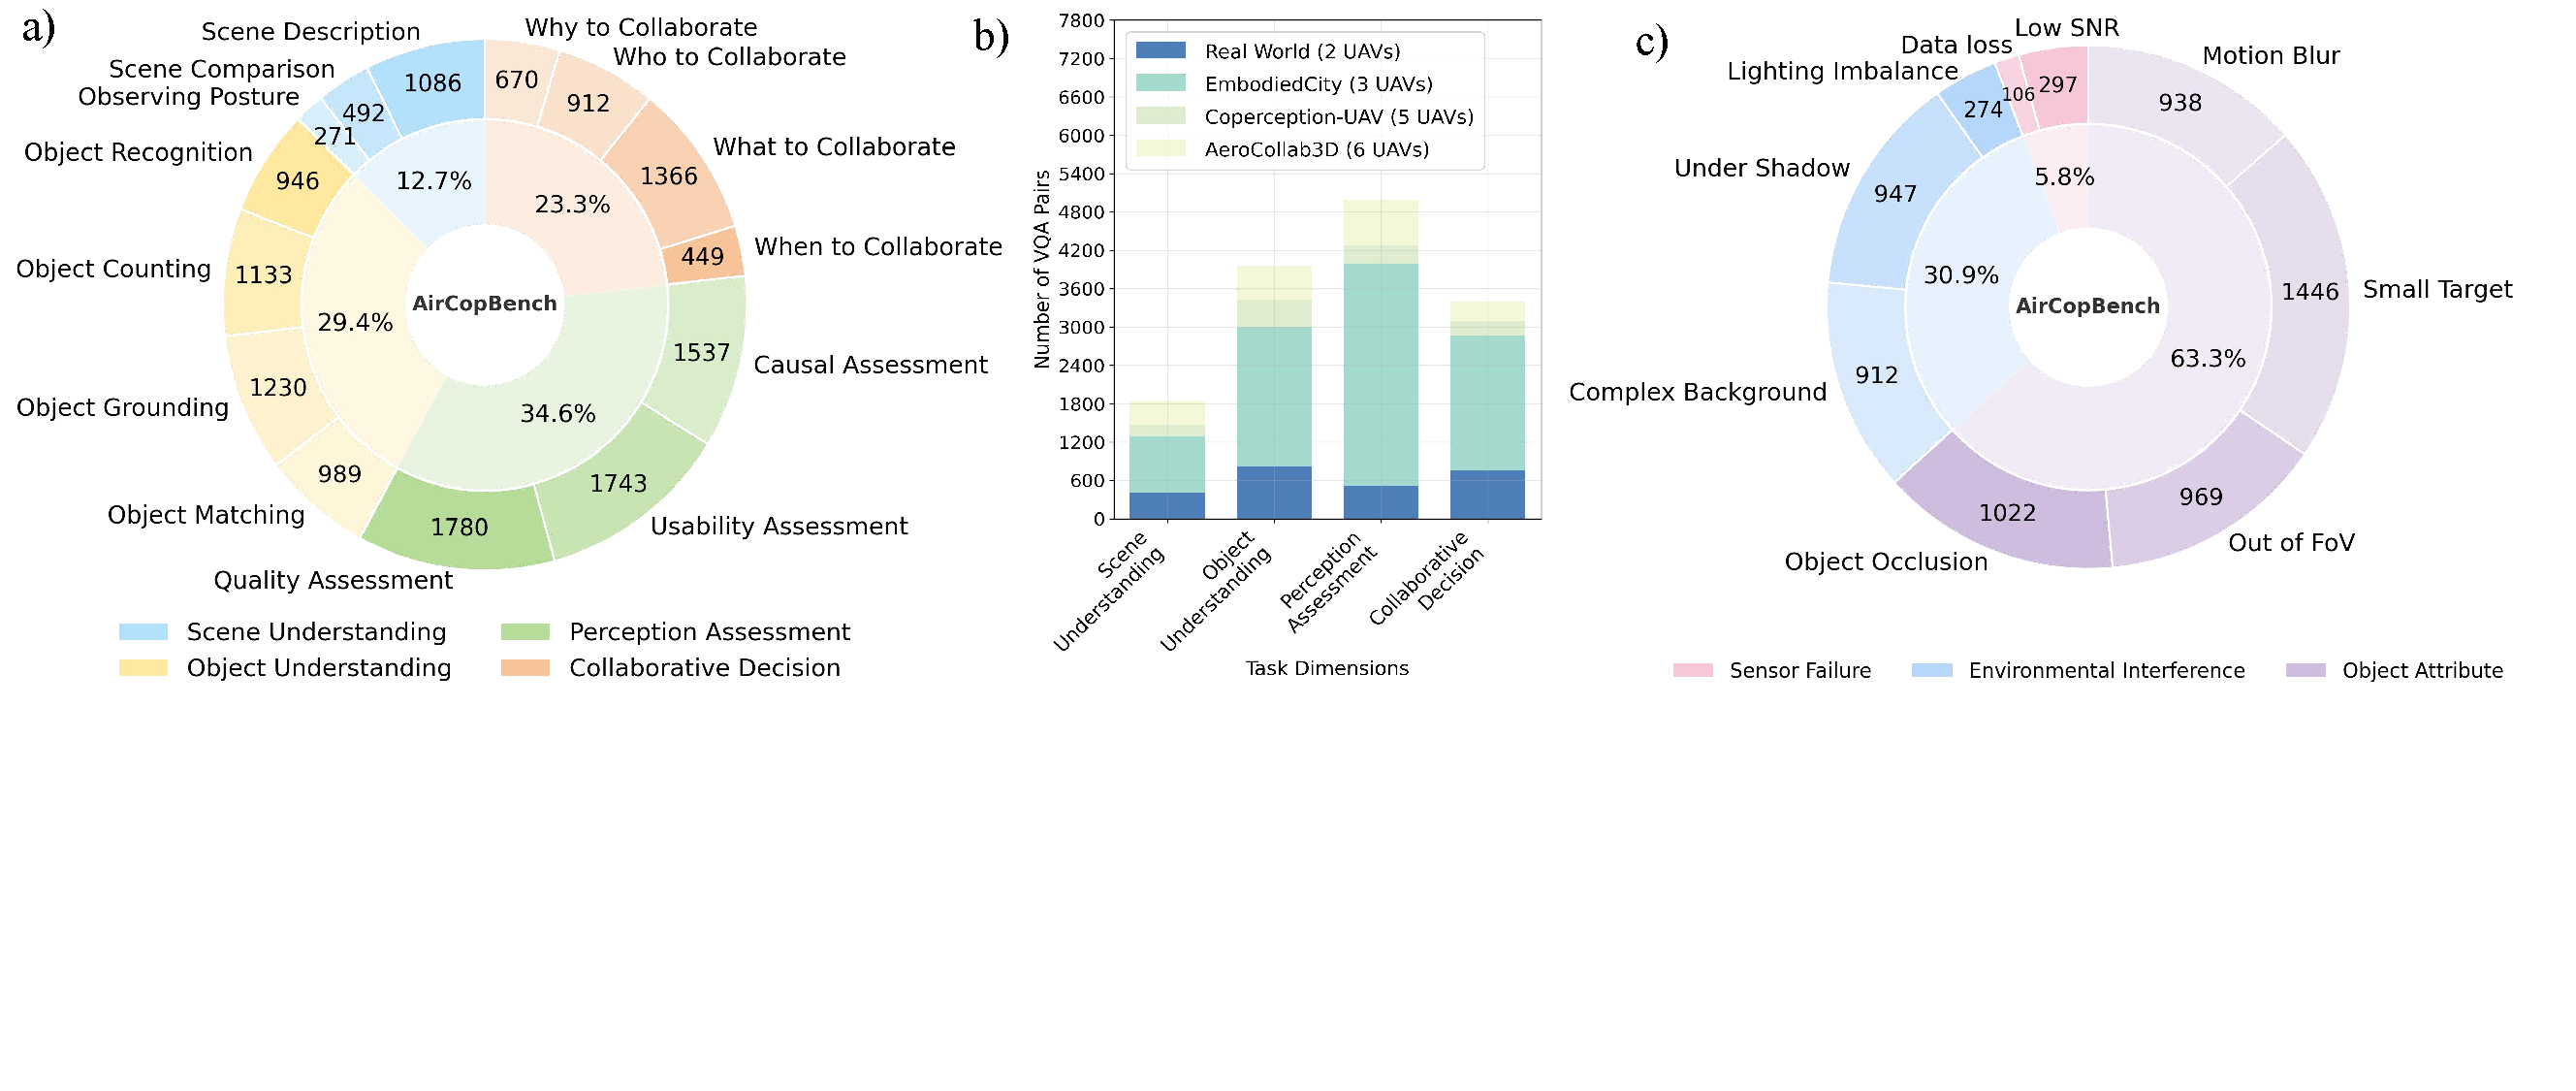
\includegraphics[width=1\linewidth]{figures/statistics.pdf}
    \caption{\textbf{Statistical Overview of AirCopBench.} a) Distribution of VQA pairs across 14 task types. b) Distribution of VQA pairs from various data sources with different numbers of observing UAV groups. c) Distribution of images featuring diverse perception degradation types.}
    \label{statistics}
    \vspace{-0.3cm}
\end{figure*}

\subsubsection{Question Generation.}
Given diverse complexity and requirements for different collaborative perception tasks, we design three approaches for question generation:
% : model-based, rule-based, and human-based generation. 
\\ \indent
\textbf{Model-based Generation.} 
This method uses powerful MLLMs, including GPT-4o \cite{hurst2024gpt} and Qwen-VL-Max-latest \cite{Qwen-VL}, to efficiently generate high-quality VQA pairs for each task. We employ four prompting techniques:
a) Task Decomposition breaks large tasks into smaller, focused tasks for better model understanding and easier debugging;
b) Role-playing Settings prompts models to generate questions from the perspective of different UAV agents in embodied perception tasks;
c) Chain-of-Thought (CoT) Prompting uses multi-step reasoning to generate complex questions requiring deep visual understanding;
d) Few-shot Learning leverages templates and examples for improved task understanding and generalization.
% This method leverages multiple powerful MLLMs, including GPT-4o \cite{hurst2024gpt} and Qwen-VL-Max-latest \cite{Qwen-VL}, to quickly produce high-quality VQA pairs for each task. Particularly, we employ four prompting techniques in this phase: 
% a) Task Decomposition, which breaks down a large generative task into smaller, independent tasks with targeted and precise prompts, enabling better model focus, understanding, and easier debugging.; 
% b) Role-playing Settings, which prompts models to generate questions from the perspective of different UAV agents in the observing system for embodied perception tasks;
% c) Chain-of-Thought (CoT) Prompting, which follows multi-step thinking process to generate complex questions that require deep visual understanding over multiple reasoning stages;
% d) Few-shot Learning, which enables models to generate questions with a few excellent question/option templates and examples for better task understanding and generalization.  
\\ \indent
\textbf{Rule-based Generation.}
This approach uses predefined rules and logic to generate structured questions. Tasks like Object Counting and Usability Assessment rely on rule-based methods, where questions are directly based on dataset annotations. These simple, deterministic rules make rule-based generation ideal for tasks requiring consistent, structured questions without complex reasoning or context.
% This approach utilizes predefined rules and logic to produce questions that follow a specific structure. For example, tasks like Object Counting and Quality Assessment rely heavily on rule-based approaches, where the questions generated are based on the predefined attributes and conditions set by the dataset from annotations. 
% % The generation process uses markup languages like XML or JSON to define rules that categorize the objects or assess the quality of the images. 
% These rules are often simple and deterministic, making rule-based generation well-suited for tasks that require structured, consistent question patterns without the need for extensive reasoning or context.
\\ \indent
\textbf{Human-based Generation.}
% This method is essential for tasks like Observing Posture and Object Matching, which require complex multi-image logical relationships and spatial understanding that models struggle to achieve. Human annotators can create questions that accurately reflect these complexities, ensuring realism and contextual richness.
% This method is essential for tasks like Observing Posture and Object Matching, which demand complex multi-image reasoning and spatial understanding—capabilities that current models often lack. By involving human experts in the annotation process, we ensure that the generated questions capture subtle visual cues, realistic scenario dynamics, and nuanced logical relationships. Their expertise enables the creation of high-quality, context-rich questions that reflect real-world challenges and human reasoning.
This method supports tasks like Observing Posture and Object Matching, which require complex multi-image reasoning and spatial understanding. Expert annotations ensure subtle visual cues, realistic dynamics, and logical nuances are well captured, yielding high-quality, context-rich questions.

% This phase also includes hybrid question generation. The detailed process and prompts can be found in the \textit{Appendix}.
% This phase also involves hybrid question generation. When model-based generation fails, rule-based generation fills the gaps, or model-based generation follows rule-based generation to enhance question variety and complexity. Furthermore, human can assist in improving machine-generated questions, enhancing efficiency and relevance.

% \subsubsection{Question Generation.}
% \begin{enumerate}[label=(\arabic*)]
%     \item Model-based generation:
%     Task decomposition.
%     CoT prompting.
%     -role-playing
%     -two-step thinking
%     -few-shot
%     \item Rule-based generation.
%     \item Human-based generation.
% \end{enumerate}

% \begin{figure*}[t]
%     \centering
%     
\includegraphics[width=1\linewidth]{AnonymousSubmission//LaTeX//figures/pipeline.pdf}
%     \caption{AirCopBench generation pipeline includes 4 main steps: Data Collection, Data Annotation, Question Generation, and Quality Control.}
%     \label{pipeline}
% \end{figure*}

\begin{table*}[t]
\centering
\caption{Results on AirCopBench for existing various MLLMs on 14 task types across 4 evaluation dimensions. The best-performing model in each category is highlighted \textbf{in-bold}, while the second-best is \underline{underlined}. 24 out of 40 models and 3 out of 4 fine-tuned models for demonstration in the main text; additional results are provided in the \textit{Appendix}.}
\label{mllms_accuracy}
\renewcommand{\arraystretch}{1.2} 
\resizebox{\textwidth}{!}{
\begin{tabular}{%
  c|cc|% 前面三列保持不变
  *{3}{>{\centering\arraybackslash}p{0.8cm}}|% 场景理解三列
  *{4}{>{\centering\arraybackslash}p{0.8cm}}|% 物体理解四列
  *{3}{>{\centering\arraybackslash}p{0.8cm}}|% 感知评估三列
  *{4}{>{\centering\arraybackslash}p{0.8cm}}  % 协作决策四列
}

\hline
& & & 
\multicolumn{3}{c|}{\cellcolor{blue!10}\textbf{Scene Understanding}} 
& \multicolumn{4}{c|}{\cellcolor{yellow!10}\textbf{Object Undstanding}} 
& \multicolumn{3}{c|}{\cellcolor{green!10}\textbf{Perception Assessment}} 
& \multicolumn{4}{c}{\cellcolor{red!10}\textbf{Collaborative Decision}} \\
\multicolumn{1}{r|}{Method} 
& Rank 
& \multicolumn{1}{c|}{Avg.} 
& \rotatebox{90}{\textit{Scene Desc.}} 
& \rotatebox{90}{\textit{Scene Comp.}} 
& \rotatebox{90}{\textit{Obs. Post.}} 
& \rotatebox{90}{\textit{Obj. Rec.}} 
& \rotatebox{90}{\textit{Obj. Cnt.}} 
& \rotatebox{90}{\textit{Obj. Grnd.}} 
& \rotatebox{90}{\textit{Obj. Mtch.}} 
& \rotatebox{90}{\textit{Qual. Ass.}} 
& \rotatebox{90}{\textit{Usab. Ass.}} 
& \rotatebox{90}{\textit{Caus. Ass.}} 
& \rotatebox{90}{\textit{When Coll.}} 
& \rotatebox{90}{\textit{What Coll.}} 
& \rotatebox{90}{\textit{Who Coll.}} 
& \rotatebox{90}{\textit{Why Coll.}} \\
\hline
\rowcolor{cyan!8}
% \rowcolor{gray!20}
\multicolumn{1}{l|}{\textbf{\textit{Baseline}}} & \multicolumn{2}{l|}{} & \multicolumn{3}{l|}{} & \multicolumn{4}{l|}{} & \multicolumn{3}{l|}{} & \multicolumn{4}{l}{} \\
% \multicolumn{17}{l}{\textbf{\textit{Baseline}}} \\
\multicolumn{1}{r|}{Random} & - & 23.47 & 19.30 & 44.19 & 18.52 & 16.67 & 23.46 & 27.68 & 17.14 & 19.51 & 19.51 & 28.57 & 41.38 & 18.52 & 24.69 & 24.69 \\
\multicolumn{1}{r|}{Human} & - & 78.25 & 71.43 & 75.86 & 42.86 & 85.71 & 88.89 & 83.04 & 87.62 & 90.48 & 91.46 & 85.71 & 51.72 & 82.72 & 82.72 & 75.31 \\
\hline
% \rowcolor{gray!20}
\rowcolor{cyan!8}
\multicolumn{1}{l|}{\textbf{\textit{Proprietary Models (API)}}} & \multicolumn{2}{l|}{} & \multicolumn{3}{l|}{} & \multicolumn{4}{l|}{} & \multicolumn{3}{l|}{} & \multicolumn{4}{l}{} \\
\multicolumn{1}{r|}{GPT-4o-2024-11-20} 
  & \cellcolor{red!50}2 & \underline{51.79} 
  & 64.91 & 55.81 & \textbf{44.44} 
  & 65.48 & \textbf{44.44} & 50.89 & \textbf{67.62} 
  & 29.76 & 48.78 & 70.24 & 34.48 & 58.02 & 14.81 & \underline{60.49} \\
\multicolumn{1}{r|}{Gemini-2.5-Pro} 
  & 5 & 49.08 
  & \underline{70.18} & 62.79 & \underline{37.04} 
  & \textbf{67.86} & 27.16 & 47.32 & 47.62 
  & 15.48 & 36.59 & \textbf{72.62} & \underline{41.38} & \underline{61.73} & \underline{34.57} & \textbf{65.43} \\
\multicolumn{1}{r|}{Claude-Sonnet-4-20250514} 
  & \cellcolor{red!10}3 & 50.73 
  & 59.65 & 55.81 & 33.33 
  & 61.90 & 33.33 & 52.68 & 56.19 
  & 35.71 & \textbf{57.32} & 71.43 & 20.69 & 60.49 & 30.86 & 51.85 \\
\multicolumn{1}{r|}{Qwen-Max-VL-latest} 
  & 4 & 50.53 
  & 52.63 & \underline{65.12} & 29.63 
  & 61.90 & \underline{41.98} & \underline{54.46} & 61.90 
  & \textbf{44.05} & 46.34 & 66.67 & 17.24 & 53.09 & \textbf{39.51} & 39.51 \\
\multicolumn{1}{r|}{Step-1o-turbo} 
  & \cellcolor{red!90}1 & \textbf{52.87} 
  & \textbf{75.00} & \textbf{70.83} & 21.05 
  & \underline{66.10} & 33.33 & \textbf{61.54} & 59.26 
  & 27.42 & \underline{55.93} & \underline{71.67} & \underline{41.38} & \textbf{67.27} & 18.52 & 56.60 \\
\multicolumn{1}{r|}{Doubao-seed-1-6-flash-250615} 
  & 2 & \underline{51.79} 
  & 59.65 & 48.84 & \underline{37.04} 
  & 54.76 & \textbf{44.44} & 53.57 & \underline{63.81} 
  & \underline{41.67} & 52.44 & 67.86 & \textbf{48.28} & 54.32 & \underline{34.57} & 48.10 \\
\hline
% \rowcolor{gray!20}
\rowcolor{cyan!8}
\multicolumn{1}{l|}{\textbf{\textit{Open-source Models}}} & \multicolumn{2}{l|}{} & \multicolumn{3}{l|}{} & \multicolumn{4}{l|}{} & \multicolumn{3}{l|}{} & \multicolumn{4}{l}{} \\
\multicolumn{1}{r|}{Phi-4-multimodal-instruct}                & 5  & 52.76    & 63.16    & 60.47    & 33.33    & 51.19    & 25.93    & 52.68    & \underline{65.71} & 26.19    & 40.24    & 70.24    & 24.14    & \textbf{66.67} & \underline{70.37} & 60.40    \\
\multicolumn{1}{r|}{Qwen2.5-VL-7B-Instruct}                   & 10 & 47.33    & \underline{66.67} & 60.47    & 25.93    & 63.10    & 25.93    & 50.89    & 51.43    & 47.56    & 47.56    & 66.67    & 13.79    & 34.57    & 25.93    & 43.21    \\
\multicolumn{1}{r|}{Qwen2.5-VL-72B-Instruct}                  & 4  & 54.90    & 59.65    & \underline{65.12} & 33.33    & 58.33    & \textbf{41.98} & \underline{63.39} & \textbf{67.62} & 48.78    & 48.78    & 73.81    & 17.24    & 59.26    & 37.04    & 48.15    \\
\multicolumn{1}{r|}{InternVL3-8B}                             & 6  & 52.18    & 56.14    & 60.47    & 25.93    & 59.52    & 30.86    & 58.04    & 56.19    & 56.10    & 51.22    & 71.43    & 20.69    & 54.32    & 53.09    & 50.62    \\
\multicolumn{1}{r|}{InternVL3-78B}                            & \cellcolor{red!10}3 & 55.38    & \underline{66.67} & \textbf{67.44} & \underline{44.44} & \underline{64.29} & 24.69    & \textbf{67.86} & 62.86    & \textbf{58.54} & \textbf{58.37} & \textbf{76.19} & 13.79    & 55.56    & 50.62    & 41.98    \\
\multicolumn{1}{r|}{Janus-Pro-7B}                             & 12 & 44.91    & 52.63    & 48.84    & 22.22    & 51.19    & 18.52    & 58.04    & 51.43    & 28.57    & 46.34    & 61.90    & 31.03    & \underline{60.49} & 33.33    & 37.00    \\
\multicolumn{1}{r|}{Chameleon-7B}                            & 15 & 38.22    & 36.84    & 37.21    & \underline{44.44} & 25.00    & 24.69    & 29.46    & 46.67    & 16.67    & 20.73    & 53.57    & 27.59    & 45.68    & \textbf{75.31} & 49.30    \\
\multicolumn{1}{r|}{PaliGemma-3B}                             & 17 & 24.25    & 19.30    & 37.21    & 22.22    & 30.95    & 35.80    & 18.75    & 13.33    & 11.90    & 21.95    & 47.62    & \textbf{65.52} & 17.28    & 16.05    & 16.05    \\
\multicolumn{1}{r|}{MiniCPM-V2.6}                             & 7  & 51.99    & 63.16    & 62.79    & 33.33    & \textbf{65.48} & \underline{40.74} & 49.11    & 49.52    & 46.43    & 48.78    & 66.67    & 41.38    & 58.02    & 46.91    & 45.68    \\
\multicolumn{1}{r|}{Ovis2-16B}                                & \cellcolor{red!90}1 & \textbf{59.17} & \textbf{68.42} & \textbf{67.44} & 29.63    & \underline{64.29} & 28.40    & 56.25    & \textbf{67.62} & \underline{58.33} & \underline{57.32} & 66.67    & \underline{51.72} & \underline{60.49} & 60.49    & \textbf{71.60} \\
\multicolumn{1}{r|}{Ovis-U1-3B}                              & 16 & 37.34    & 57.89    & 46.51    & 22.22    & 41.67    & 29.63    & 36.61    & 39.05    & 27.38    & 45.12    & 63.10    & 24.14    & 24.69    & 29.63    & 25.93    \\
\multicolumn{1}{r|}{Kimi-VL-A3B-Thinking}                     & \cellcolor{red!50}2 & \underline{56.84} & 59.65    & 60.47    & 25.93    & 61.90    & 38.27    & 58.04    & 63.81    & 45.24    & 50.00    & \textbf{76.19} & 48.28    & \textbf{66.67} & 51.85    & \underline{62.96} \\
\multicolumn{1}{r|}{Mimo-VL-7B-RL}                            & 9  & 48.59    & 61.40    & 58.14    & 29.63    & \underline{64.29} & 34.57    & 53.57    & 57.14    & 46.43    & 53.66    & \underline{75.00} & 10.34    & 50.62    & 17.28    & 33.33    \\
\multicolumn{1}{r|}{LLaVA-NeXT-7B-hf}                        & 14 & 38.31    & 28.07    & 46.51    & 18.52    & 35.71    & 25.93    & 39.29    & 52.38    & 29.76    & 37.80    & 59.52    & 27.59    & 55.56    & 25.93    & 29.63    \\
\multicolumn{1}{r|}{LLaVA-NeXT-13B-hf}                       & 13 & 39.28    & 31.58    & 44.19    & 33.33    & 42.86    & 30.86    & 40.18    & 46.67    & 40.48    & 41.46    & 50.00    & 34.48    & 44.44    & 34.57    & 24.69    \\
\multicolumn{1}{r|}{Skywork-R1V3}                             & 8  & 48.94    & 46.15    & 43.33    & \textbf{46.67} & 41.51    & 40.00    & 50.00    & 46.99    & 40.74    & 56.60    & 67.27    & 33.33    & 52.94    & 48.08    & 51.92    \\
\multicolumn{1}{r|}{mPLUG-OWL3}                              & 11 & 47.14    & 57.89    & 60.47    & 22.22    & 50.00    & 25.93    & 56.25    & 41.90    & 27.38    & 47.56    & 55.95    & 44.83    & 54.32    & 50.62    & 54.32    \\
\multicolumn{1}{r|}{XComposer-VL-7B}                         & 18 & 23.26    & 14.81    & 20.00    & 18.75    & 25.45    & 26.42    & 18.82    & 22.62    & 27.78    & 13.79    & 13.79    & 12.50    & 24.07    & 39.62    & 33.96    \\
\hline
% \rowcolor{gray!20}
\rowcolor{cyan!8}
\multicolumn{1}{l|}{\textbf{\textit{Fine-tuned Models}}} & \multicolumn{2}{l|}{} & \multicolumn{3}{l|}{} & \multicolumn{4}{l|}{} & \multicolumn{3}{l|}{} & \multicolumn{4}{l}{} \\
\multicolumn{1}{r|}{LLaVA-NeXT-13B} & \cellcolor{red!10}3  & 57.61        & 40.35        & \underline{60.47} & \underline{25.93} & 52.38        & \underline{45.68} & \underline{59.82} & 60.95        & 57.14        & 62.20        & 69.05        & \underline{37.93} & \underline{58.02} & 70.37        & 66.67        \\
\multicolumn{1}{r|}{Qwen-2.5-VL-7B} & \cellcolor{red!90}1          & \textbf{74.30} & \underline{63.16} & \textbf{65.12}  & \textbf{33.33}    & \textbf{69.05} & \textbf{75.31}    & \textbf{66.07}    & \textbf{72.38} & \textbf{76.19} & \textbf{82.93} & \textbf{83.33} & \textbf{55.17}    & \textbf{77.78} & \textbf{91.36} & \textbf{85.10} \\
\multicolumn{1}{r|}{Qwen-2.5-VL-3B} & \cellcolor{red!50}2 & \underline{66.44} & \textbf{73.68} & 55.81           & \textbf{33.33}    & \underline{59.52} & 34.57             & 57.14             & \underline{62.86} & \underline{66.67} & \underline{73.17} & \underline{82.14} & \textbf{55.17}    & \textbf{77.78} & \underline{90.12} & \underline{80.20}  \\
\hline
\rowcolor{cyan!8}
\multicolumn{1}{l|}{\textbf{\textit{Sim-to-Real Experiments}}} & \multicolumn{2}{l|}{} & \multicolumn{3}{l|}{} & \multicolumn{4}{l|}{} & \multicolumn{3}{l|}{} & \multicolumn{4}{l}{} \\
\multicolumn{1}{r|}{Qwen2.5-VL-7B}  
  & - & 47.77 & 50.00 & 55.56 & 11.11 & 83.33 & 50.00 & 27.78 & 55.56 & 61.11 & 44.44 & 82.35 & 10.53 & 38.89 & 64.71 & 27.70 \\
\multicolumn{1}{r|}{AirCop-7B} & -  & 67.41 & 50.00 & 77.78 & 11.11 & 83.33 & 88.89 & 77.78 & 77.78 & 77.78 & 94.44 & 82.35 & 31.58 & 50.00 & 76.47 & 50.00 \\
\hline
\end{tabular}
}
\end{table*}


\subsubsection{Quality Control.}
To ensure the reliability and effectiveness of our dataset for training and evaluating models on collaborative perception, we implement three key quality control measures: Standard Examination, Blind Filtering, and Human Refinement. 
\\ \indent
\textbf{Standard Examination.} 
This measure evaluates the quality of generated VQA pairs based on four criteria:
a) Required Content ensures all necessary information is included, flagging incomplete pairs for revision;
b) Format Consistency maintains uniform structure, wording, and presentation;
c) Answer Validity checks the correctness and relevance of options, filtering out incorrect ones and ensuring the correct option is present;
d) Question Length ensures questions are sufficiently detailed to avoid ambiguity.
% This measure evaluates the quality of generated VQA pairs according to a set of fixed scoring criteria, including four main indicators: 
% a) Required Content ensures each VQA pair includes all necessary information, flagging incomplete content for revision;
% b) Format Consistency mandates uniformity in structure, wording, and presentation across the dataset;
% c) Answer Validity checks the correctness and relevance of answer choices, filtering out clearly incorrect options and ensuring the presence of the correct option;
% d) Question Length ensures questions are of adequate length to avoid ambiguity.
\\ \indent
\textbf{Blind Filtering.}
This measure aims to remove questions answerable through common sense by using n MLLMs to predict answers without the multi-view image input. If all MLLMs answer correctly, the question is removed, filtering out invalid questions that can be answered solely through general perception knowledge \cite{zhao2025urbanvideo}.
\\ \indent
\textbf{Human Refinement.}
This step further ensures human modification of generated questions with issues such as:
a) Ambiguous Questions that are unclear, poorly framed, or irrelevant to the perception task;
b) Invalid Options that are missing correct answers, contain duplicates or mismatched content;
c) Incorrect Answers that are missing, contain multiple selections when only one is required, or are incorrectly chosen.
% a) Ambiguous Question: The question is unclear, poorly framed, or irrelevant to the perception task;
% b) Invalid Options: Answer choices lack a correct option, include duplicates, or not match the multi-view image content;
% c) Incorrect Answers: The correct answer is missing, incorrectly selected, or multiple answers may be chosen when only one is required.
The entire human refinement process takes over 800 hours. Specific modified examples are provided in \textit{Appendix}.

% This step further ensures the human modification of generated questions that still exhibit the following issues:
% a) Ambiguous Question: The question is unclear, poorly framed, or irrelevant to the perception task;
% b) Invalid Options: Answer choices lack a correct option, include duplicates, or not match the multi-view image content;
% c) Incorrect Answers: The correct answer is missing, incorrectly selected, or multiple answers may be chosen when only one is required.
% % These issues arise from three main sources that still exist in current advanced MLLMs for multi-UAV collaborative perception tasks:
% % a) Element perception hallucination in the scene;
% % b) Limited spatial reasoning capability;
% % c) Deficient multi-image understanding ability.
% The whole refinement process costs over 800 hours. Specific modification examples are provided in \textit{Appendix}.

% \subsubsection{Quality Control.}
% \begin{enumerate}[label=(\arabic*)]
%     \item Standard examination: Scoring criterion:
% required content
% format consistency
% answer validity
% question length 

%     \item Blind filtering.
%     \item Human refinement.
% \end{enumerate}


\subsection{Benchmark Statistics} 
AirCopBench comprises 2,920 simultaneous multi-view images with various challenging perception degradation collected from real world and simulators, as shown in Fig.~\ref{statistics}b\&c. The dataset includes 14,610 questions, including both basic tasks like scene and object understanding, as well as advanced tasks like perception assessment and collaborative decision, as detailed in Fig.~\ref{statistics}a. 
% The training set and the test set contain approximately 13.2k and 1.1k questions, respectively. More statistical details can be found in Appendix.

% 1058 test

\section{Experiments}
This section introduces the evaluated models and protocols, evaluates 40 mainstream MLLMs on AirCopBench, and summarizes results across model types. It also analyzes task correlations, sim-to-real potential, and error cases.
% It further analyzes capability correlations between tasks and sim-to-real potential, and categorizes error causes across tasks.

\subsection{Experimental Setup}
\subsubsection{Evaluation Metric.}
We integrate AirCopBench evaluation into the VLMEvalKit~\cite{duan2024vlmevalkit} framework, enabling capability assessments of new MLLMs. Specifically, we measure MLLM accuracy for each task type using question-answering accuracy.
% We integrate the evaluation of AirCopBench into the standard VLMEvalKit~\cite{duan2024vlmevalkit} framework, thereby facilitating subsequent capability assessments of newly developed MLLMs. Specifically, we calculate the accuracy of MLLMs for each task type using question answering accuracy.
\subsubsection{Baselines.}
We conduct zero-shot evaluations of 40 MLLMs on AirCopBench in Tab.~\ref{mllms_accuracy}. The baselines include both proprietary models, such as GPT-4o \cite{hurst2024gpt}, Gemini-2.5-Pro \cite{comanici2025gemini}, Claude-Sonnet-4~\cite{Claude3S}, and Qwen-Max-VL~\cite{Qwen-VL}, as well as open-source models capable of multi-image input, including LLaVA series \cite{liu2024llavanext}, Qwen-VL series \cite{bai2025qwen2, wang2024qwen2} and Phi series~\cite{abdin2024phi3, abdin2024phi4}, among others. Additional evaluated models include~\cite{chen2025janus, lu2023chameleon, yao2024minicpm, team2025kimi, Yue2025MiMoVLTR, ye2024mplugowl2, shen2025skywork, lu2024ovis,wang2025ovis, beyer2024paligemma, zhu2025internvl3}.

% \subsubsection{Others.} 
% All local model inference and finetuning is performed on 4$\times$ A800-SXM4-80GB. Details of the baseline settings and prompts can be found in \textit{Appendix}.

% \subsection{Main Results}
\subsection{Model Comparison}
From the quantitative results shown in Tab.~\ref{mllms_accuracy}, we have the following findings:

\begin{itemize}[left=0pt]
    \item \textbf{AirCopBench poses significant challenges to all MLLMs.}
    Both proprietary and open-source models perform poorly on aerial collaborative perception tasks, with the best model, Ovis-16B~\cite{lu2024ovis}, achieving only 59.17\% accuracy. This highlights the importance of AirCopBench in revealing the insufficient development of embodied perception and collaborative decision-making abilities in current MLLMs.

    \item \textbf{Leading open-source MLLMs match or exceed the best proprietary models on AirCopBench.}
    Models like Ovis2-16B~\cite{lu2024ovis} and Kimi-VL-A3B-Thinking~\cite{team2025kimi} match or slightly surpass top proprietary systems. However, the overall performance gap remains modest, and both open-source and proprietary MLLMs still struggle with multi-image understanding, underscoring the need for further progress in multi-image reasoning.
    
    % Models like Ovis2-16B~\cite{lu2024ovis} and Kimi-VL-A3B-Thinking~\cite{team2025kimi} perform on par with or slightly better than top proprietary systems. However, the performance gap between open-source and proprietary MLLMs is modest, with both struggling to fully address the challenges of multi-image understanding, highlighting persistent limitations in current multi-image reasoning.
    
    % Models such as Ovis2-16B~\cite{lu2024ovis} and Kimi-VL-A3B-Thinking~\cite{team2025kimi} achieve performance on par with—or even slightly better than—flagship closed-source systems. However, the average performance difference between open-source and proprietary MLLMs is modest, and neither category fully overcomes the inherent difficulties of multi-image understanding, indicating persistent limitations in current multi-image reasoning capabilities.

    % \item \textbf{Parameter scale affects the performance of MLLMs on AirCopBench.}
    % Smaller parameter models appear to be more unstable. For two models with equivalent average accuracy, the open-source small parameter model tends to have a lower minimum accuracy across all tasks compared to the commercial large parameter model.

    \item \textbf{MLLMs demonstrate a clear bias across various question categories.}
    Current MLLMs perform well on tasks like Scene Description and Scene Comparison, but struggle with categories requiring domain knowledge and goal-oriented reasoning, such as Usability Assessment and When to Collaborate. This indicates a need for significant improvements in embodied perception assessment and adaptive collaboration decision-making.
    % Current MLLMs perform relatively well on the ``Scene Description" and ``Scene Comparison", while exhibit poor performance on categories that require prior professional knowledge and task-oriented analysis, such as ``Usability Assessment" and ``When to Collaborate". This suggests that MLLMs still need significant improvement in their ability to perform embodied perception assessment and adaptive collaboration decision-making.
\end{itemize}

% \subsection{Detailed Analysis}
\subsection{Correlation Analysis}
\begin{figure}[t]
    \centering
    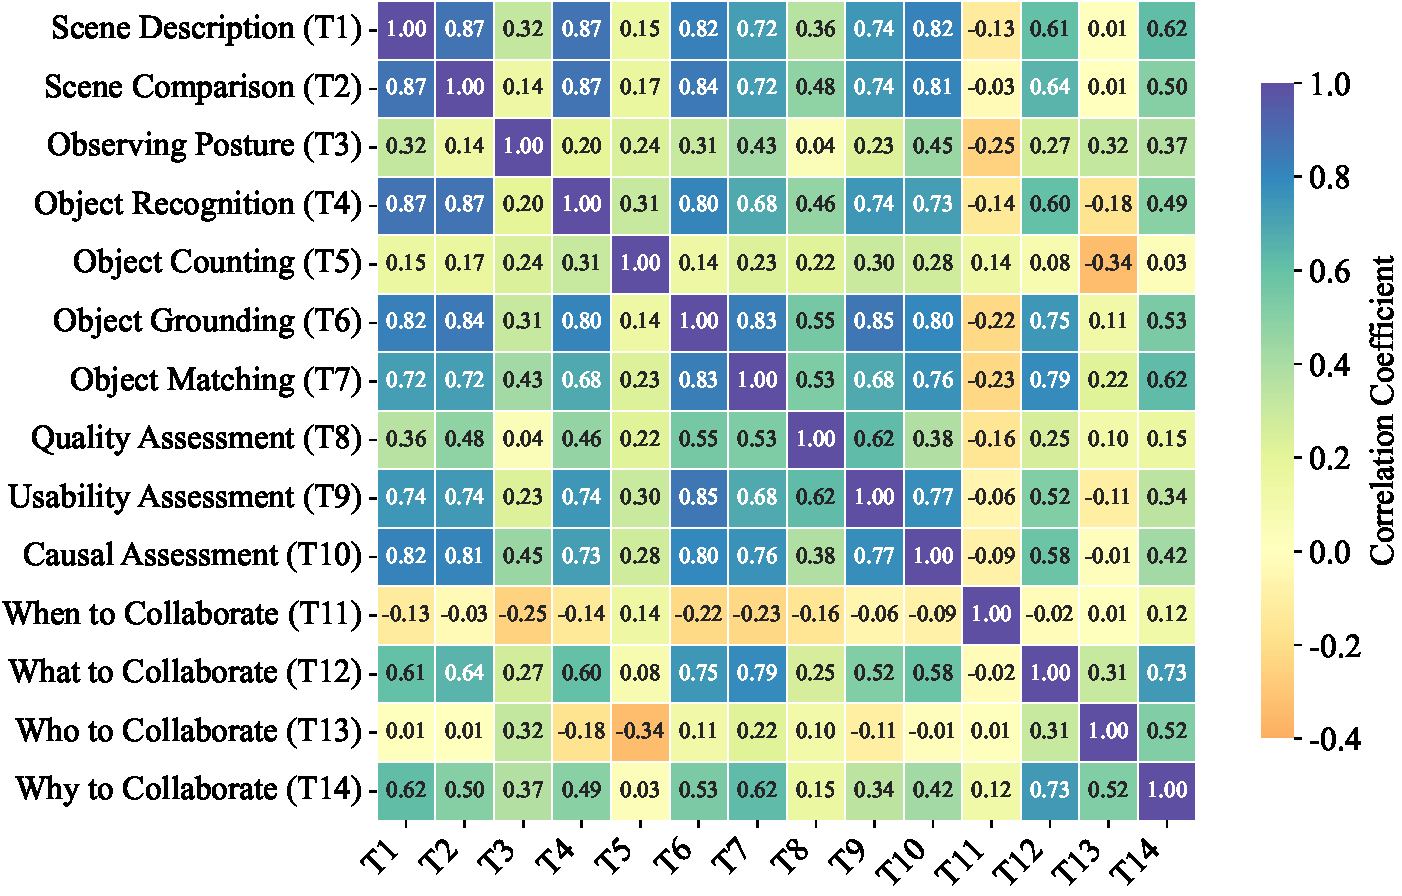
\includegraphics[width=1\linewidth]
    {figures/correlation.pdf}
    \caption{Correlation coefficients of MLLMs' performance across all tasks, with higher values indicating greater similarity in the cognitive abilities required by the two tasks.}
    \label{correlation}
    \vspace{-0.3cm}
\end{figure}
To explore the relationships between tasks and their required cognitive abilities, we compute pairwise correlations of MLLMs' accuracy (Tab.~\ref{comparison}) on each task. Similar performance across models on two tasks suggests shared cognitive abilities. From Fig.~\ref{correlation}, we draw the following conclusions:
\begin{itemize}[left=0pt]
    \item \textbf{Causal Assessment exhibits a high correlation with almost all other tasks.} It suggests that understanding and inferring the causality of perception degradation is crucial for various cognitive processes. This finding implies that causal assessment could be a key factor in the development of embodied cognition in collaborative perception.
    % \item \textbf{Object-centric tasks demonstrate strong inter-correlations among themselves.} These tasks all involve object-related information, implying the cognitive ability to share underlying requirement for these tasks.
    \item \textbf{Object Matching has a high correlation with both Object Recognition and Object Grounding tasks.} This observation aligns with prior knowledge that effective multi-view image understanding relies on strong single-image perceptual capabilities.
    % \item \textbf{When to Collaborate exhibits low correlations with other task types.} This task relies on distinct cognitive processes not shared with the other tasks in our analysis, suggesting that certain embodied cognitive abilities may function independently rather than as part of a general intelligence framework. Therefore, tasks involving these high-level collaborative abilities require targeted training.
    \item \textbf{Quality Assessment exhibits moderate correlations with multiple tasks.} This suggests that quality evaluation requires integrating Scene Understanding, Object Recognition, and Object Matching abilities, making it a highly composite decision‐making task.
\end{itemize}

\subsection{Supervised Fine-Tuning}
We fine-tune two representative MLLMs, Qwen-2.5-VL (7B and 3B)~\cite{bai2025qwen2} and LLaVA-NeXT-13B~\cite{liu2024llavanext}, using our curated instruction dataset within the LLaMA-Factory framework~\cite{zheng2024llamafactory}, with default hyperparameters for three epochs. As shown in Tab.~\ref{mllms_accuracy}, Qwen-2.5-VL-7B achieves 74.30\% accuracy (+26.97), Qwen-2.5-VL-3B reaches 66.44\% (+19.11), and LLaVA-NeXT-13B improves to 57.61\% (+19.30), demonstrating that domain-specific SFT substantially enhances MLLM performance in collaborative perception.

% We apply SFT to two widely used MLLM architectures, Qwen-2.5-VL (7B and 3B)~\cite{bai2025qwen2} and LLaVA-NeXT-13B~\cite{liu2024llavanext}, using our curated instruction dataset within the LLaMA-Factory framework~\cite{zheng2024llamafactory}, retaining default hyperparameters and training for three epochs. As shown in Tab.~\ref{mllms_accuracy}, Qwen-2.5-VL-7B achieves 74.30\% overall accuracy (+26.97 points), Qwen-2.5-VL-3B reaches 66.44\% (+19.11 points), and LLaVA-NeXT-13B improves to 57.61\% (+19.30 points). These results confirm that SFT with domain-specific instructions significantly boosts MLLM performance in collaborative perception tasks.

% We apply SFT to two widely used MLLM architectures—Qwen-2.5-VL (7B and 3B)~\cite{bai2025qwen2} and LLaVA-NeXT-13B~\cite{liu2024llavanext}—using our curated instruction dataset within the LLaMA-Factory framework~\cite{zheng2024llamafactory}, retaining default hyperparameters and training for three epochs. As shown in Tab.~\ref{mllms_accuracy}, Qwen-2.5-VL–7B improves to 74.30\% overall accuracy (a +26.97-point gain over its pre-trained baseline), Qwen-2.5-VL–3B reaches 66.44\% (+19.11 points), and LLaVA-NeXT-13B climbs to 57.61\% (+19.30 points). Overall, these results confirm that SFT with domain-specific instructions substantially enhances MLLM performance across diverse collaborative perception tasks.

\subsection{Sim-to-Real}
We evaluate the generalization of models trained on simulated data to real-world UAV imagery. As shown in Tab.~\ref{mllms_accuracy}, we compare the open-source Qwen2.5-VL-7B~\cite{bai2025qwen2} and our AirCop-7B model fine-tuned on simulator data. Qwen2.5-VL-7B achieves 47.77\% overall accuracy, performing well in Object Recognition (83.33\%) but poorly in Posture (11.11\%) and Collaboration (40\%). After fine-tuning, AirCop-7B reaches 67.41\% (+19.64), with notable gains in Object Grounding (77.78\%, +50.00), Object Counting (88.89\%, +38.89), and Usability Assessment (94.44\%, +53.20). These results confirm that simulator-based fine-tuning significantly enhances sim-to-real transfer, improving generalization to real UAV imagery and validating the effectiveness of our simulated dataset.

% We evaluate the ability of models trained on simulated data to generalize to real-world UAV imagery. Tab.\ref{mllms_accuracy} shows two key configurations on the real-world test split: the open-source Qwen2.5-VL-7B\cite{bai2025qwen2} model applied directly, and our AirCop-7B model fine-tuned on simulator data. Qwen2.5-VL-7B scores 47.77\% overall, excelling in Object Recognition (83.33\%) but underperforming in Posture (11.11\%) and Collaboration (40\%). After fine-tuning on simulated data, AirCop-7B achieves 67.41\% (+19.64\%), with significant improvements in Object Grounding (77.78\%, +50.00\%), Object Counting (88.89\%, +38.89\%), and Usability Assessment (94.44\%, +53.20\%). These results demonstrate that fine-tuning on our simulated data enhances sim-to-real transfer, enabling the AirCop-7B model to generalize effectively to real UAV imagery and confirming the value of our simulated dataset for real-world UAV perception tasks.
% We further evaluate the ability of models trained on simulated data to generalize to real-world UAV imagery. Tab.~\ref{mllms_accuracy} reports two key configurations on the real-world test split: the open-source Qwen2.5-VL-7B~\cite{bai2025qwen2} model applied directly, and our AirCop-7B model fine-tuned on simulator data and then tested on real images. On the real‐world split, Qwen2.5-VL-7B~\cite{bai2025qwen2} scores 47.77\% overall, showing strong Object Recognition (83.33\%) but weak Posture (11.11\%) and Collaboration (40\%) performance. After fine-tuning on simulated data, AirCop-7B achieves 67.41\% (+19.64\%), with notable gains in Object Grounding (77.78\%, +50.00\%), Object Counting (88.89\%, +38.89\%) and Usability Assessment (94.44\%, +53.20\%). These results confirm that fine-tuning on our simulated dataset yields strong sim-to-real transfer: the AirCop-7B model learns robust object- and collaboration-level reasoning that carries over to real UAV imagery, validating the utility of our simulated data for real‐world UAV perception tasks.

\subsection{Error Analysis}
The errors in MLLM reasoning primarily stem from three causes, as shown in Fig.~\ref{error}:
\begin{figure}
    \centering
    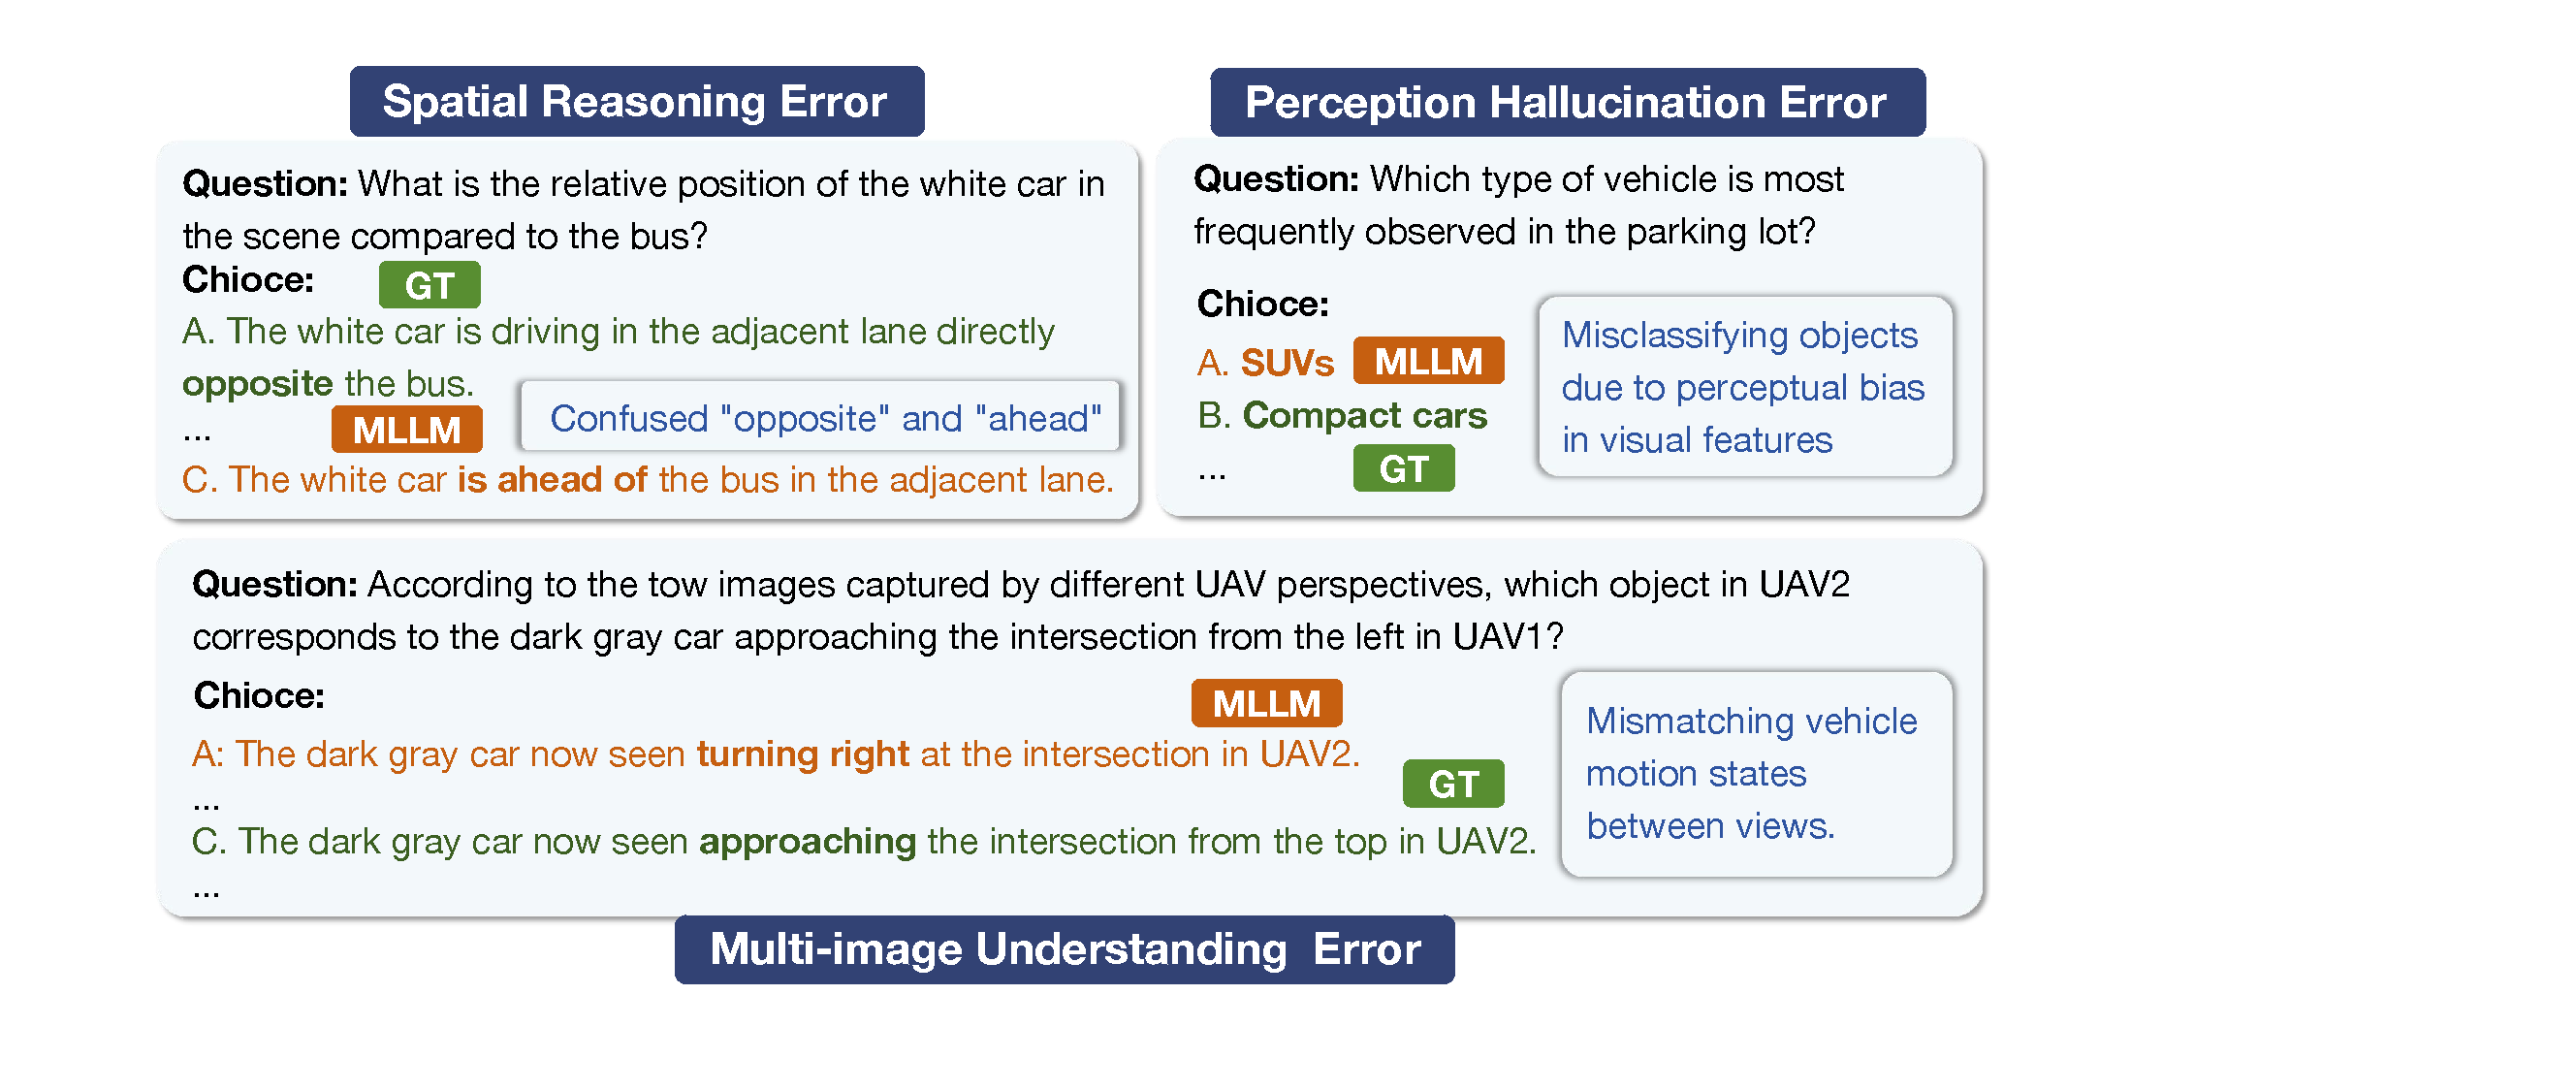
\includegraphics[width=1\linewidth]{figures/error.pdf}
    \caption{Examples of three common errors in MLLM reasoning during aerial collaborative perception tasks.}
    \label{error}
    \vspace{-0.3cm}
\end{figure}
\begin{itemize}[left=0pt]
    \item \textbf{Perception hallucination errors.} 
    MLLMs misidentify or fail to recognize objects due to perception hallucination, where visual input is incorrectly processed, leading to false or exaggerated perceptions of objects.
    % MLLMs can suffer from perception hallucination, where they incorrectly identify or fail to recognize objects in the images. This occurs when the model's visual processing capabilities lead to false or exaggerated perceptions, causing incorrect object recognition or misinterpretation of visual elements. For example, a model might identify a non-existent object or misclassify an object due to ambiguities in the visual input or inherent biases in the model's training data.
    
    \item \textbf{Spatial reasoning errors.}
    MLLMs struggle with spatial reasoning, causing errors in interpreting object relationships, such as incorrect positioning or orientation of objects in space \cite{zhang2025point, zha2025enable}.
    % MLLMs may struggle with spatial reasoning, which is essential for accurately interpreting the relationships between objects in space. Limited spatial understanding can lead to errors in reasoning about the relative positions, orientations, or distances between objects. For instance, a model might incorrectly infer that an object is in front of another when it is actually behind, or fail to recognize a spatially complex scene due to inadequate reasoning capabilities.
    
    \item \textbf{Multi-image understanding errors.} 
    MLLMs face challenges in multi-image understanding, resulting in errors when comparing, matching, or integrating information across images, leading to incorrect logical inferences.
    % MLLMs often face difficulties in multi-image understanding, which involves comparing and integrating information across multiple images. This limitation can result in errors when the model needs to assess logical relationships or contrasts between images. For example, a model may fail to correctly compare objects across two images, misinterpret changes between them, or overlook contextual cues that are essential for accurate reasoning, leading to incorrect answers in multi-image VQA tasks.
\end{itemize}
Perceptual and spatial errors hinder Object Recognition and Grounding, while multi-image reasoning limits Scene Comparison, Object Matching, and Collaborative Decision; other tasks show varied failure modes (see \textit{Appendix}).
% Object Recognition and Grounding are hindered by perceptual hallucinations and spatial errors. Scene Comparison, Object Matching, and Collaborative Decision face multi-image understanding issues, while other complex tasks encounter various errors. See \textit{Appendix} for more details.

% Object Recognition and Grounding tasks, reliant on visual abilities, suffer from perception hallucination and spatial reasoning errors. Scene Comparison, Object Matching, and Collaborative Decision suffer from multi-image understanding errors. As for the complex and challenging tasks, such as perception assessment and collaborative analysis, various errors are prevalent. See \textit{Appendix} for more analysis and cases.

\section{Conclusion}
% In this work, we present AirCopBench, a benchmark for multi-UAV collaborative perception under challenging degradations, comprising 2.9k+ multi-view images and 14.6k+ questions. We evaluate 40 mainstream MLLMs across scene understanding, object understanding, perception assessment, and collaborative decision-making. The best-performing models achieve only 59.17\% accuracy, highlighting challenges in multi-view collaborative perception, revealing significant challenges in collaborative perception and task-specific biases. Fine-tuning with simulated data improves real-world performance. Future work will expand to more diverse real-world data and develop efficient MLLM architectures for practical multi-UAV deployment.

In this work, we propose AirCopBench, a benchmark for multi-UAV collaborative perception with challenging degradation, featuring 2.9k+ multi-view images and 14.6k+ questions. We evaluate 40 popular MLLMs on scene understanding, object understanding, perception assessment, and collaborative decision. The best-performing models achieve only 59.17\% a ccuracy, highlighting challenges in multi-view collaborative perception. Their performance also shows biases across task types. Fine-tuned MLLMs with simulated data improves their performance on real-world tasks. Future work will extend to more diverse real-world data and explore efficient MLLM architectures for practical multi-UAV deployment.

\section{Acknowledgments}
This paper was supported by the Natural Science Foundation of China under Grant 62371269, Shenzhen Low-Altitude Airspace Strategic Program Portfolio Z253061 and Meituan Academy of Robotics Shenzhen. Sponsored by Tsinghua University-Toyota Research Center.


\bibliography{aaai2026}

\end{document}
